\documentclass[../dw-oefeningen.tex]{subfiles}
\begin{document}
\chapter{Inleiding tot de grafentheorie}

% \section*{Theorie}
\section*{Oefeningen}

\begin{enumerate}
  \item Professor McBrain en zijn echtgenote April geven een feestje waar
        nog vier andere koppels op uit genodigd zijn. Sommige mensen schudden 
        elkaar de hand, maar uiteraard niet hun eigen partner. Op het
        eind van het feestje vraagt McBrain aan alle gasten en aan zijn vrouw
        aan hoeveel mensen ze een hand hebben gegeven, en hij krijgt negen
        verschillende antwoorden. Hoeveel mensen hebben een hand gegeven
        aan April?

        \hrulefill

        9 verschillende antwoorden betekent dat de graad van de 9 toppen 
        verschillend is.

        Er zijn 10 mensen. De persoon zelf en de partner vallen af, dus 
        er kunnen maximum 8 personen de hand geschud worden. De mogelijke 
        antwoorden liggen dus tussen 0 en 8, 9 verschillende antwoorden:
        
        \begin{center}
        \begin{tikzpicture}
          \node[circle, fill=black, inner sep=2pt, label=90:P] (nP) at (90:2.5) {};
          \node[circle, fill=black, inner sep=2pt, label=54:8] (n8) at (54:2.5) {};
          \node[circle, fill=black, inner sep=2pt, label=18:7] (n7) at (18:2.5) {};
          \node[circle, fill=black, inner sep=2pt, label=-18:6] (n6) at (-18:2.5) {};
          \node[circle, fill=black, inner sep=2pt, label=-54:5] (n5) at (-54:2.5) {};
          \node[circle, fill=black, inner sep=2pt, label=-90:4] (n4) at (-90:2.5) {};
          \node[circle, fill=black, inner sep=2pt, label=-126:3] (n3) at (-126:2.5) {};
          \node[circle, fill=black, inner sep=2pt, label=-162:2] (n2) at (-162:2.5) {};
          \node[circle, fill=black, inner sep=2pt, label=162:1] (n1) at (162:2.5) {};
          \node[circle, fill=black, inner sep=2pt, label=126:0] (n0) at (126:2.5) {};
        \end{tikzpicture}
        \end{center}

        De persoon die 8 mensen de hand heeft geschud, heeft iedereen de hand 
        geschud, behalve:
        \begin{itemize}
          \item zichzelf
          \item de persoon die 0 mensen de hand heeft geschud
        \end{itemize}
        
        \begin{center}
        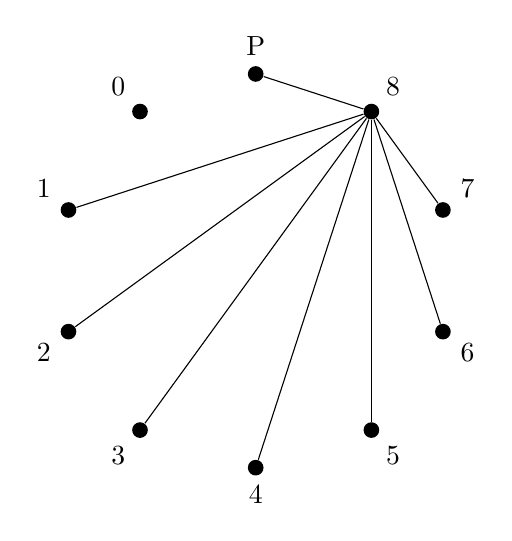
\begin{tikzpicture}
          \node[circle, fill=black, inner sep=2pt, label=90:P] (nP) at (90:2.5) {};
          \node[circle, fill=black, inner sep=2pt, label=54:8] (n8) at (54:2.5) {};
          \node[circle, fill=black, inner sep=2pt, label=18:7] (n7) at (18:2.5) {};
          \node[circle, fill=black, inner sep=2pt, label=-18:6] (n6) at (-18:2.5) {};
          \node[circle, fill=black, inner sep=2pt, label=-54:5] (n5) at (-54:2.5) {};
          \node[circle, fill=black, inner sep=2pt, label=-90:4] (n4) at (-90:2.5) {};
          \node[circle, fill=black, inner sep=2pt, label=-126:3] (n3) at (-126:2.5) {};
          \node[circle, fill=black, inner sep=2pt, label=-162:2] (n2) at (-162:2.5) {};
          \node[circle, fill=black, inner sep=2pt, label=162:1] (n1) at (162:2.5) {};
          \node[circle, fill=black, inner sep=2pt, label=126:0] (n0) at (126:2.5) {};
          
          \draw (n8) -- (nP);
          \draw (n8) -- (n7);
          \draw (n8) -- (n6);
          \draw (n8) -- (n5);
          \draw (n8) -- (n4);
          \draw (n8) -- (n3);
          \draw (n8) -- (n2);
          \draw (n8) -- (n1);
        \end{tikzpicture}
        \end{center}

        Het eerste koppel dat we kunnen identificeren, is dus het koppel \((8, 0)\).

        Top 7 mag niet verbonden worden met:
        \begin{itemize}
          \item zichzelf
          \item de persoon die 0 mensen de hand heeft geschud
          \item de persoon die 1 persoon de hand heeft geschud, want die is al verbonden
                met 8
        \end{itemize}

        \begin{center}
        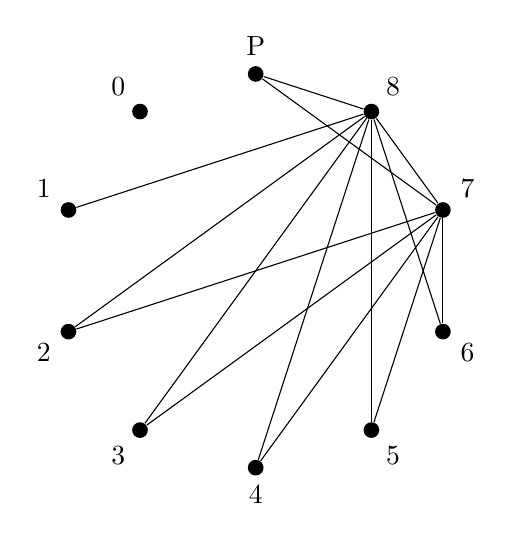
\begin{tikzpicture}
          \node[circle, fill=black, inner sep=2pt, label=90:P] (nP) at (90:2.5) {};
          \node[circle, fill=black, inner sep=2pt, label=54:8] (n8) at (54:2.5) {};
          \node[circle, fill=black, inner sep=2pt, label=18:7] (n7) at (18:2.5) {};
          \node[circle, fill=black, inner sep=2pt, label=-18:6] (n6) at (-18:2.5) {};
          \node[circle, fill=black, inner sep=2pt, label=-54:5] (n5) at (-54:2.5) {};
          \node[circle, fill=black, inner sep=2pt, label=-90:4] (n4) at (-90:2.5) {};
          \node[circle, fill=black, inner sep=2pt, label=-126:3] (n3) at (-126:2.5) {};
          \node[circle, fill=black, inner sep=2pt, label=-162:2] (n2) at (-162:2.5) {};
          \node[circle, fill=black, inner sep=2pt, label=162:1] (n1) at (162:2.5) {};
          \node[circle, fill=black, inner sep=2pt, label=126:0] (n0) at (126:2.5) {};
          
          \draw (n8) -- (nP);
          \draw (n8) -- (n7);
          \draw (n8) -- (n6);
          \draw (n8) -- (n5);
          \draw (n8) -- (n4);
          \draw (n8) -- (n3);
          \draw (n8) -- (n2);
          \draw (n8) -- (n1);
          
          \draw (n7) -- (nP);
          \draw (n7) -- (n6);
          \draw (n7) -- (n5);
          \draw (n7) -- (n4);
          \draw (n7) -- (n3);
          \draw (n7) -- (n2);
        \end{tikzpicture}
        \end{center}

        Het tweede koppel dat we kunnen identificeren, is dus het koppel \((7, 1)\).

        Dit kan verder met 6:
        \begin{center}
        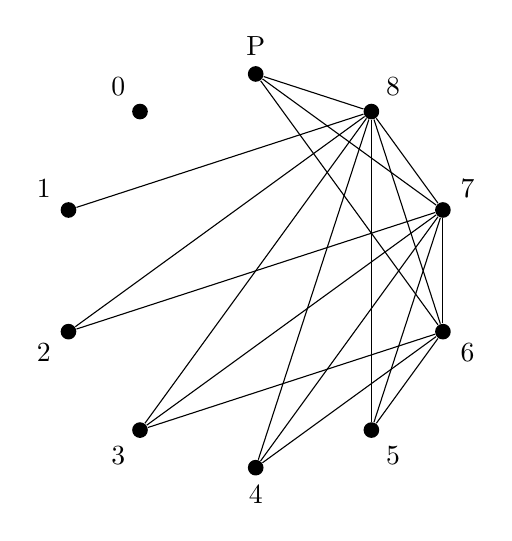
\begin{tikzpicture}
          \node[circle, fill=black, inner sep=2pt, label=90:P] (nP) at (90:2.5) {};
          \node[circle, fill=black, inner sep=2pt, label=54:8] (n8) at (54:2.5) {};
          \node[circle, fill=black, inner sep=2pt, label=18:7] (n7) at (18:2.5) {};
          \node[circle, fill=black, inner sep=2pt, label=-18:6] (n6) at (-18:2.5) {};
          \node[circle, fill=black, inner sep=2pt, label=-54:5] (n5) at (-54:2.5) {};
          \node[circle, fill=black, inner sep=2pt, label=-90:4] (n4) at (-90:2.5) {};
          \node[circle, fill=black, inner sep=2pt, label=-126:3] (n3) at (-126:2.5) {};
          \node[circle, fill=black, inner sep=2pt, label=-162:2] (n2) at (-162:2.5) {};
          \node[circle, fill=black, inner sep=2pt, label=162:1] (n1) at (162:2.5) {};
          \node[circle, fill=black, inner sep=2pt, label=126:0] (n0) at (126:2.5) {};
          
          \draw (n8) -- (nP);
          \draw (n8) -- (n7);
          \draw (n8) -- (n6);
          \draw (n8) -- (n5);
          \draw (n8) -- (n4);
          \draw (n8) -- (n3);
          \draw (n8) -- (n2);
          \draw (n8) -- (n1);
          
          \draw (n7) -- (nP);
          \draw (n7) -- (n6);
          \draw (n7) -- (n5);
          \draw (n7) -- (n4);
          \draw (n7) -- (n3);
          \draw (n7) -- (n2);
          
          \draw (n6) -- (nP);
          \draw (n6) -- (n5);
          \draw (n6) -- (n4);
          \draw (n6) -- (n3);
        \end{tikzpicture}
        \end{center}

        Het derde koppel is dus \((6, 2)\).
        
        Dit kan verder met 6:
        \begin{center}
        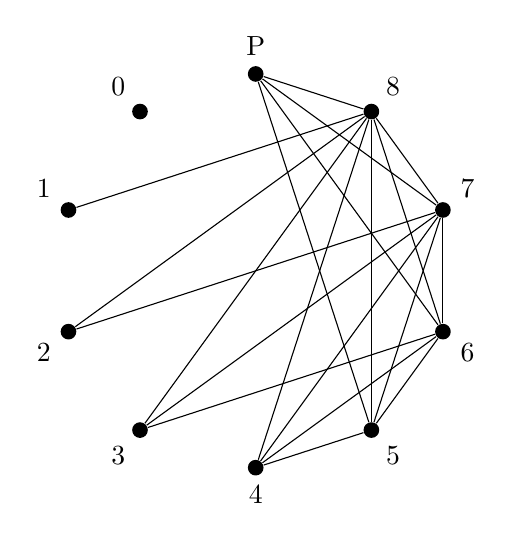
\begin{tikzpicture}
          \node[circle, fill=black, inner sep=2pt, label=90:P] (nP) at (90:2.5) {};
          \node[circle, fill=black, inner sep=2pt, label=54:8] (n8) at (54:2.5) {};
          \node[circle, fill=black, inner sep=2pt, label=18:7] (n7) at (18:2.5) {};
          \node[circle, fill=black, inner sep=2pt, label=-18:6] (n6) at (-18:2.5) {};
          \node[circle, fill=black, inner sep=2pt, label=-54:5] (n5) at (-54:2.5) {};
          \node[circle, fill=black, inner sep=2pt, label=-90:4] (n4) at (-90:2.5) {};
          \node[circle, fill=black, inner sep=2pt, label=-126:3] (n3) at (-126:2.5) {};
          \node[circle, fill=black, inner sep=2pt, label=-162:2] (n2) at (-162:2.5) {};
          \node[circle, fill=black, inner sep=2pt, label=162:1] (n1) at (162:2.5) {};
          \node[circle, fill=black, inner sep=2pt, label=126:0] (n0) at (126:2.5) {};
          
          \draw (n8) -- (nP);
          \draw (n8) -- (n7);
          \draw (n8) -- (n6);
          \draw (n8) -- (n5);
          \draw (n8) -- (n4);
          \draw (n8) -- (n3);
          \draw (n8) -- (n2);
          \draw (n8) -- (n1);
          
          \draw (n7) -- (nP);
          \draw (n7) -- (n6);
          \draw (n7) -- (n5);
          \draw (n7) -- (n4);
          \draw (n7) -- (n3);
          \draw (n7) -- (n2);
          
          \draw (n6) -- (nP);
          \draw (n6) -- (n5);
          \draw (n6) -- (n4);
          \draw (n6) -- (n3);
          
          \draw (n5) -- (nP);
          \draw (n5) -- (n4);
        \end{tikzpicture}
        \end{center}

        Het vierde koppel is dus \((5, 3)\).

        De geïdentificeerde koppels zijn dus:
        \begin{align*}
          \begin{tabular}{cc}
            8 & 0 \\
            7 & 1 \\
            6 & 2 \\
            5 & 3 
          \end{tabular}
        \end{align*}

        Het laatste overblijvende koppel is dan \((P, 4)\), de professor en April.

        April heeft dus \textbf{4} mensen de hand geschud.
\end{enumerate}

\begin{enumerate}[start=7]
  \item Zeg van de volgende lijsten van getallen of het de graden kunnen zijn
        van de toppen van een graaf. Zo ja, teken een graaf die eraan voldoet.

        \begin{enumerate}
          \item 2, 2, 2, 3
          \item 2, 2, 4, 4, 4
          \item 1, 2, 2, 3, 4
          \item 1, 2, 3, 4
        \end{enumerate}

        \hrulefill

        
        \begin{enumerate}
          \item 2, 2, 2, 3
          
                Handshake principe:
                \[
                  \sum_{v \in V(\mathcal{G})} \deg(v) = 2 | E(\mathcal{G}) |
                \]

                De som van de graden is dus altijd even. Hier is de som \(2 + 2 + 2 + 3 = 9\),
                wat oneven is. Deze graaf kan dus niet bestaan.

          \item 2, 2, 4, 4, 4
          
                De som van de toppen is even, dus daarmee kunnen we het al niet uitsluiten.

                De drie toppen van graad 4 moeten elk verbonden zijn met de vier andere toppen, 
                dus ook met de twee toppen van graad 2. Die zouden dus minstens graad 3 moeten hebben.

                Deze graaf kan dus niet bestaan.

          \item 1, 2, 2, 3, 4
          
                De som van de toppen is even, dus daarmee kunnen we het al niet uitsluiten.

                \begin{center}
                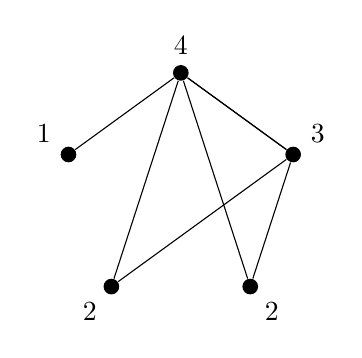
\begin{tikzpicture}
                  \node[circle, fill=black, inner sep=2pt, label=90:4] (n4) at (90:1.5) {};
                  \node[circle, fill=black, inner sep=2pt, label=18:3] (n3) at (18:1.5) {};
                  \node[circle, fill=black, inner sep=2pt, label=-54:2] (n2b) at (-54:1.5) {};
                  \node[circle, fill=black, inner sep=2pt, label=-126:2] (n2) at (-126:1.5) {};
                  \node[circle, fill=black, inner sep=2pt, label=162:1] (n1) at (162:1.5) {};

                  \draw (n4) -- (n1);
                  \draw (n4) -- (n2);
                  \draw (n4) -- (n2b);
                  \draw (n4) -- (n3);
                  
                  \draw (n3) -- (n2);
                  \draw (n3) -- (n2b);
                  \draw (n3) -- (n4);
                  
                \end{tikzpicture}
                \end{center}

                Deze graaf is dus mogelijk.
                
          \item 1, 2, 3, 4
          
                De som van de toppen is even, dus daarmee kunnen we het al niet uitsluiten.

                Deze graaf kan niet bestaan om 2 redenen:

                \begin{enumerate}
                  \item een graaf waarvan de toppen alle een verschillende graad hebben,
                        kan niet bestaan;
                  \item de top met graad 4 moet met 4 andere toppen verbonden worden, maar er zijn 
                        slechts 3 andere toppen.
                \end{enumerate}
                
                
        \end{enumerate}
\end{enumerate}

\begin{enumerate}[start=11]
  \item Toon aan: als \(\mathcal{G}\) een simpele graaf is met minstens 2 toppen, dan
        heeft \(\mathcal{G}\) 2 toppen van dezelfde graad. 

        \hrulefill

        Een simpele graaf is een graaf zonder lussen.

        Voor een graaf met \(n\) toppen, ligt de graad van de toppen tussen

        \[ 0 \le \deg(v) \le n - 1\]

        Dat zijn \(n\) verschillende mogelijkheden. Het duiventilprincipe kan dus niet
        toegepast worden.

        Maar: als elke top een andere graad heeft, zal elk van de graden precies één 
        keer moeten voorkomen.
      
        \begin{center}
        \begin{tikzpicture}
          \node[circle, fill=black, inner sep=2pt, label=90:$n - 1$] (nm1) at (90:2.5) {};
          \node[circle, fill=black, inner sep=2pt, label=54:$\dots$] (ndots) at (54:2.5) {};
          \node[circle, fill=black, inner sep=2pt, label=18:7] (n7) at (18:2.5) {};
          \node[circle, fill=black, inner sep=2pt, label=-18:6] (n6) at (-18:2.5) {};
          \node[circle, fill=black, inner sep=2pt, label=-54:5] (n5) at (-54:2.5) {};
          \node[circle, fill=black, inner sep=2pt, label=-90:4] (n4) at (-90:2.5) {};
          \node[circle, fill=black, inner sep=2pt, label=-126:3] (n3) at (-126:2.5) {};
          \node[circle, fill=black, inner sep=2pt, label=-162:2] (n2) at (-162:2.5) {};
          \node[circle, fill=black, inner sep=2pt, label=162:1] (n1) at (162:2.5) {};
          \node[circle, fill=black, inner sep=2pt, label=126:0] (n0) at (126:2.5) {};
        \end{tikzpicture}
        \end{center}

        \(n - 1\) mag niet met zichzelf verbonden zijn, en moet dus met al de andere 
        toppen verbonden zijn, ook met \(0\). Dit is een tegenspraak.

\end{enumerate}

Een \textit{Eulergraf} bevat een gesloten pad dat elke \textbf{boog} precies één keer passeert.
Deze graf mag ook nog andere bogen bevatten. Een graf (zonder geïsoleerde toppen) is een Eulergraf als:
\begin{itemize}
  \item de toppen allemaal een even graad hebben;
  \item de graf samenhangend is.
\end{itemize}

De buitenste toppen van de laatste graf hebben graad 1:

\begin{center}
\begin{tikzpicture}
  % First graph - square
  \begin{scope}[xshift=0cm]
    \node[circle, fill=black, inner sep=2pt] (a1) at (0,1) {};
    \node[circle, fill=black, inner sep=2pt] (a2) at (1,1) {};
    \node[circle, fill=black, inner sep=2pt] (a3) at (1,0) {};
    \node[circle, fill=black, inner sep=2pt] (a4) at (0,0) {};
    
    \draw (0,1) -- (1,1) -- (1,0) -- (0,0) -- cycle;
  \end{scope}

  \begin{scope}[xshift=4cm]
    \draw (0,1) -- (1,0.5) -- (2,1) -- (2,0) -- (1,0.5) -- (0,0) -- cycle;
    
    \node[circle, fill=black, inner sep=2pt] (c1) at (0,1) {};
    \node[circle, fill=black, inner sep=2pt] (c2) at (1,0.5) {};
    \node[circle, fill=black, inner sep=2pt] (c3) at (2,1) {};
    \node[circle, fill=black, inner sep=2pt] (c4) at (2,0) {};
    \node[circle, fill=black, inner sep=2pt] (c5) at (0,0) {};
  \end{scope}

  \begin{scope}[xshift=8cm]
    \node at (1,-1) {geen};

    % Draw edges from center to all outer nodes
    \draw ($(1,0.5)+(0:0)$) -- ($(1,0.5)+(90:0.8)$);
    \draw ($(1,0.5)+(0:0)$) -- ($(1,0.5)+(30:0.8)$);
    \draw ($(1,0.5)+(0:0)$) -- ($(1,0.5)+(-30:0.8)$);
    \draw ($(1,0.5)+(0:0)$) -- ($(1,0.5)+(-90:0.8)$);
    \draw ($(1,0.5)+(0:0)$) -- ($(1,0.5)+(-150:0.8)$);
    \draw ($(1,0.5)+(0:0)$) -- ($(1,0.5)+(150:0.8)$);
    
    % Draw nodes
    \node[circle, fill=black, inner sep=2pt] at (1,0.5) {};
    \node[circle, fill=black, inner sep=2pt] at ($(1,0.5)+(90:0.8)$) {};
    \node[circle, fill=black, inner sep=2pt] at ($(1,0.5)+(30:0.8)$) {};
    \node[circle, fill=black, inner sep=2pt] at ($(1,0.5)+(-30:0.8)$) {};
    \node[circle, fill=black, inner sep=2pt] at ($(1,0.5)+(-90:0.8)$) {};
    \node[circle, fill=black, inner sep=2pt] at ($(1,0.5)+(-150:0.8)$) {};
    \node[circle, fill=black, inner sep=2pt] at ($(1,0.5)+(150:0.8)$) {};
  \end{scope}
\end{tikzpicture}
\end{center}



Een \textit{Hamiltongraf} bevat een gesloten pad dat elke \textbf{top} precies één keer passeert.
Deze graf mag ook nog andere bogen bevatten.

\begin{center}
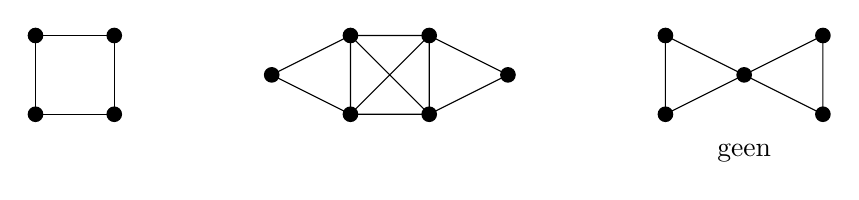
\begin{tikzpicture}
  % First graph - square
  \begin{scope}[xshift=0cm]
    \node[circle, fill=black, inner sep=2pt] (a1) at (0,1) {};
    \node[circle, fill=black, inner sep=2pt] (a2) at (1,1) {};
    \node[circle, fill=black, inner sep=2pt] (a3) at (1,0) {};
    \node[circle, fill=black, inner sep=2pt] (a4) at (0,0) {};
    
    \draw (0,1) -- (1,1) -- (1,0) -- (0,0) -- cycle;
  \end{scope}
  
  % Second graph - pentagon with all diagonals
  \begin{scope}[xshift=4cm]
    \draw (-1,0.5) -- (0,1) -- (1,1) -- (2,0.5) -- (1,0) -- (0,0) -- cycle;
    \draw (0,1) -- (1,0) -- (1,1) -- (0,0) -- cycle;
    
    \node[circle, fill=black, inner sep=2pt] (b1) at (-1,0.5) {};
    \node[circle, fill=black, inner sep=2pt] (b2) at (0,1) {};
    \node[circle, fill=black, inner sep=2pt] (b3) at (1,1) {};
    \node[circle, fill=black, inner sep=2pt] (b4) at (2,0.5) {};
    \node[circle, fill=black, inner sep=2pt] (b5) at (1,0) {};
    \node[circle, fill=black, inner sep=2pt] (b6) at (0,0) {};
  \end{scope}
  
  % Third graph - bowtie with label "geen"
  \begin{scope}[xshift=8cm]
    \node at (1,-0.5) {geen};
    
    \draw (0,1) -- (1,0.5) -- (2,1) -- (2,0) -- (1,0.5) -- (0,0) -- cycle;
    
    \node[circle, fill=black, inner sep=2pt] (c1) at (0,1) {};
    \node[circle, fill=black, inner sep=2pt] (c2) at (1,0.5) {};
    \node[circle, fill=black, inner sep=2pt] (c3) at (2,1) {};
    \node[circle, fill=black, inner sep=2pt] (c4) at (2,0) {};
    \node[circle, fill=black, inner sep=2pt] (c5) at (0,0) {};
  \end{scope}
\end{tikzpicture}
\end{center}

\begin{enumerate}[start=12]
  \item 
  
        \begin{center}
        \begin{tikzpicture}
          % Draw edges first
          % Front face
          \draw (0,0) -- (2,0) -- (2,2) -- (0,2) -- cycle;
          % Back face
          \draw (1,0.5) -- (3,0.5) -- (3,2.5) -- (1,2.5) -- cycle;
          % Connecting edges
          \draw (0,0) -- (1,0.5);
          \draw (2,0) -- (3,0.5);
          \draw (2,2) -- (3,2.5);
          \draw (0,2) -- (1,2.5);

          \draw[pad-pijl] (0,0) -- (0,2);
          \draw[pad-pijl] (0,2) -- (1,2.5);
          \draw[pad-pijl] (1,2.5) -- (3,2.5);
          \draw[pad-pijl] (3,2.5) -- (2,2);
          \draw[pad-pijl] (2,2) -- (2,0);
          \draw[pad-pijl] (2,0) -- (3,0.5);
          \draw[pad-pijl] (3,0.5) -- (1,0.5);
          \draw[pad-pijl] (1,0.5) -- (0,0);
          
          
          % Draw nodes on top
          % Front face vertices
          \node[circle, fill=black, inner sep=2pt] at (0,0) {};
          \node[circle, fill=black, inner sep=2pt] at (2,0) {};
          \node[circle, fill=black, inner sep=2pt] at (2,2) {};
          \node[circle, fill=black, inner sep=2pt] at (0,2) {};
          % Back face vertices
          \node[circle, fill=black, inner sep=2pt] at (1,0.5) {};
          \node[circle, fill=black, inner sep=2pt] at (3,0.5) {};
          \node[circle, fill=black, inner sep=2pt] at (3,2.5) {};
          \node[circle, fill=black, inner sep=2pt] at (1,2.5) {};
        \end{tikzpicture}
        \end{center}
\end{enumerate}

\begin{center}
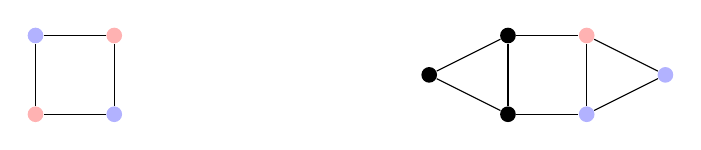
\begin{tikzpicture}
  % First graph - K_{2,2}
  \begin{scope}
    \node[circle, fill=blue!30, inner sep=2pt] (a1) at (0,1) {};
    \node[circle, fill=red!30 , inner sep=2pt] (a2) at (0,0) {};
    \node[circle, fill=red!30,  inner sep=2pt] (b1) at (1,1) {};
    \node[circle, fill=blue!30, inner sep=2pt] (b2) at (1,0) {};
    
    \draw (a1) -- (b1) -- (b2) -- (a2) -- (a1);
  \end{scope}

  % Second graph - pentagon-like structure
  \begin{scope}[xshift=5cm]
    \node[circle, fill=black,   inner sep=2pt] (n1) at (0,0.5) {};
    \node[circle, fill=black,   inner sep=2pt] (n2) at (1,1) {};
    \node[circle, fill=black,   inner sep=2pt] (n3) at (1,0) {};
    \node[circle, fill=red!30,  inner sep=2pt] (n4) at (2,1) {};
    \node[circle, fill=blue!30, inner sep=2pt] (n5) at (2,0) {};
    \node[circle, fill=blue!30, inner sep=2pt] (n6) at (3,0.5) {};
    
    \draw (n1) -- (n2);
    \draw (n1) -- (n3);

    \draw (n2) -- (n3);
    \draw (n2) -- (n4);
    \draw (n3) -- (n5);

    \draw (n4) -- (n5);
    \draw (n4) -- (n6);
    \draw (n5) -- (n6);
  \end{scope}
\end{tikzpicture}
\end{center}

In een bipartiete graf kan je telkens van kleur wisselen. Rechts is er een probleem
omdat er een lus van oneven lengte is.

\begin{enumerate}[start=13]
  % Oefening 13
  \item Elke top stelt een kubus voor. Het is een bipartiete graf aangezien we buren alternerend
        kunnen inkleuren. In totaal zijn er 27 toppen. We zoeken dus een 
        Hamiltonpad van lengte 26 (aantal bogen). In een bipartiete graf eindigt een pad van 
        even lengte altijd in dezelfde kleur (rood \(\to\) groen \(\to\) rood).

        De muis kan dus niet in het midden van de kubus eindigen.
        \begin{center}
          \includegraphics[width=0.6\textwidth]{../images/4-13.png}
        \end{center}
\end{enumerate}




\begin{enumerate}[start=15]
  % Oefening 15
  \item Waar of onwaar?
        \begin{enumerate}
          \item Als een graaf een Eulercyclus heeft, dan heeft hij een even aantal bogen.
          
                Onwaar. Bij een driehoek hebben de toppen graad 2, maar zijn er een
                oneven aantal bogen.
                \begin{center}
                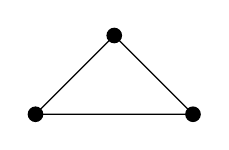
\begin{tikzpicture}
                  \draw (0,0) -- (1,1) -- (2,0) -- cycle;

                  \node[circle, fill=black, inner sep=2pt] at (0,0) {};
                  \node[circle, fill=black, inner sep=2pt] at (1,1) {};
                  \node[circle, fill=black, inner sep=2pt] at (2,0) {};
                \end{tikzpicture}
                \end{center}

          \item Zij \(\mathcal{G}\) een simpele graaf met 9 toppen en veronderstel dat de som
                van alle graden minstens 27 is. Dan heeft \(\mathcal{G}\) een top met graad
                minstens 4.

                Volgens de Handshake-eigenschap, moet het totaal aantal graden even zijn.
                De som moet dus minstens \textbf{28} zijn.

                Het is een simpele graf, dus elke top kan met 0 tot en met 8 andere toppen
                verbonden zijn. Dat zijn 9 mogelijkheden.

                Als elke top met 3 andere toppen verbonden is, is het totaal \(3 \cdot 9 = 27\).
                Het totaal aantal graden, moet echter even zijn. Een totaal van 28 kunnen we 
                niet halen met een maximum van graad 3.

                De uitspraak is dus waar.

          \item Het aantal mensen dat een oneven aantal broers en zussen heeft, is even.
          
                Anders gesteld: het aantal toppen van oneven graad is even.

                Handshake:
                \begin{align*}
                  &\sum_{v \in V(\mathcal{G})} \deg(v) \text{ is even}
                  &\\[1em]
                  &V(\mathcal{G}) = \underbrace{E}_\text{even graad} \cup \underbrace{O}_\text{oneven graad} \\
                  &\underbrace{\sum_{v \in V(\mathcal{G})} \deg(v)}_\text{is even}
                    = \underbrace{\sum_{v \in E} \deg(v) }_\text{som van even getallen is even}
                      + \underbrace{\sum_{v \in O} \deg(v)}_\text{moet dus ook even zijn}
                  %
                \end{align*}
                
                De som van oneven getallen kan enkel even zijn als het aantal getallen even is.
                Het aantal elementen in \(O\) moet dus even zijn.

                De uitspraak is dus waar.
                

          \item Als een simpele graaf een Eulercyclus heeft, dan heeft hij ook een
                Hamiltoncyclus.

                \begin{center}
                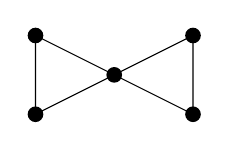
\begin{tikzpicture}

                  \begin{scope}
                    \draw (0,1) -- (1,0.5) -- (2,1) -- (2,0) -- (1,0.5) -- (0,0) -- cycle;
                    
                    \node[circle, fill=black, inner sep=2pt] (c1) at (0,1) {};
                    \node[circle, fill=black, inner sep=2pt] (c2) at (1,0.5) {};
                    \node[circle, fill=black, inner sep=2pt] (c3) at (2,1) {};
                    \node[circle, fill=black, inner sep=2pt] (c4) at (2,0) {};
                    \node[circle, fill=black, inner sep=2pt] (c5) at (0,0) {};
                  \end{scope}

                \end{tikzpicture}
                \end{center}

                Dit is een Eulergraf, maar geen Hamilotongraf. De uitspraak is dus niet waar.

          \item Als een simpele graaf een Hamiltoncyclus heeft, dan heeft hij ook
                een Eulercyclus.

                \begin{center}
                \begin{tikzpicture}
                  % Draw edges first
                  % Front face
                  \draw (0,0) -- (2,0) -- (2,2) -- (0,2) -- cycle;
                  % Back face
                  \draw (1,0.5) -- (3,0.5) -- (3,2.5) -- (1,2.5) -- cycle;
                  % Connecting edges
                  \draw (0,0) -- (1,0.5);
                  \draw (2,0) -- (3,0.5);
                  \draw (2,2) -- (3,2.5);
                  \draw (0,2) -- (1,2.5);

                  \draw[pad-pijl] (0,0) -- (0,2);
                  \draw[pad-pijl] (0,2) -- (1,2.5);
                  \draw[pad-pijl] (1,2.5) -- (3,2.5);
                  \draw[pad-pijl] (3,2.5) -- (2,2);
                  \draw[pad-pijl] (2,2) -- (2,0);
                  \draw[pad-pijl] (2,0) -- (3,0.5);
                  \draw[pad-pijl] (3,0.5) -- (1,0.5);
                  \draw[pad-pijl] (1,0.5) -- (0,0);
                  
                  
                  % Draw nodes on top
                  % Front face vertices
                  \node[circle, fill=black, inner sep=2pt] at (0,0) {};
                  \node[circle, fill=black, inner sep=2pt] at (2,0) {};
                  \node[circle, fill=black, inner sep=2pt] at (2,2) {};
                  \node[circle, fill=black, inner sep=2pt] at (0,2) {};
                  % Back face vertices
                  \node[circle, fill=black, inner sep=2pt] at (1,0.5) {};
                  \node[circle, fill=black, inner sep=2pt] at (3,0.5) {};
                  \node[circle, fill=black, inner sep=2pt] at (3,2.5) {};
                  \node[circle, fill=black, inner sep=2pt] at (1,2.5) {};
                \end{tikzpicture}
                \end{center}
                
                Deze is wel een Hamiltongraf, maar geen Eulergraf.

          \item In een reguliere graaf heeft elke top niet alleen hetzelfde aantal
                buren maar ook hetzelfde aantal toppen op afstand 2.

                De afstand is de lengte van het \textbf{kortste} pad tussen twee toppen.

                Een reguliere graaf is een graaf waarbij alle toppen dezelfde graad hebben.

                \begin{center}
                \begin{tikzpicture}
                  % First graph - square
                  \begin{scope}[xshift=0cm]
                    \node[circle, fill=black, inner sep=2pt] (a1) at (0,1) {};
                    \node[circle, fill=black, inner sep=2pt] (a2) at (1,1) {};
                    \node[circle, fill=black, inner sep=2pt] (a3) at (1,0) {};
                    \node[circle, fill=black, inner sep=2pt] (a4) at (0,0) {};
                    
                    \draw (0,1) -- (1,1) -- (1,0) -- (0,0) -- cycle;
                  \end{scope}

                  \begin{scope}[xshift=4cm]
                    \draw ($(1,0.5)+(90:0.8)$) -- ($(1,0.5)+(18:0.8)$) -- ($(1,0.5)+(-54:0.8)$) -- ($(1,0.5)+(-126:0.8)$) -- ($(1,0.5)+(162:0.8)$) -- cycle;
                    
                    % Draw nodes
                    \node[circle, fill=black, inner sep=2pt] at ($(1,0.5)+(90:0.8)$) {};
                    \node[circle, fill=black, inner sep=2pt] at ($(1,0.5)+(18:0.8)$) {};
                    \node[circle, fill=black, inner sep=2pt] at ($(1,0.5)+(-54:0.8)$) {};
                    \node[circle, fill=black, inner sep=2pt] at ($(1,0.5)+(-126:0.8)$) {};
                    \node[circle, fill=black, inner sep=2pt] at ($(1,0.5)+(162:0.8)$) {};

                  \end{scope}

                \end{tikzpicture}
                \end{center}
                
                Als we dit als één graf beschouwen, bestaande uit twee onsamenhangende componenten, 
                dan hebben de toppen van het vierkant één top op afstand 2. De toppen van de vijfhoek 
                hebben twéé toppen op afstand 2.

                De uitspraak is dus onwaar.

                Ook voor een samenhangende graf geldt dit:
                \begin{center}
                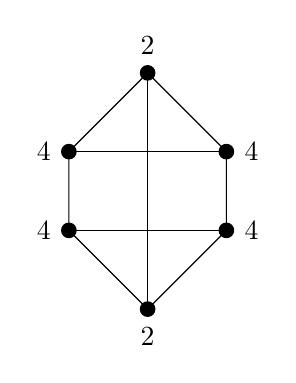
\begin{tikzpicture}
                  \begin{scope}
                    \draw (0,0) -- (0,1) 
                      -- (1,2) 
                      -- (2,1) -- (2,0)
                      -- (1,-1)
                      -- cycle;
                    \draw (0,0) -- (2,0);
                    \draw (0,1) -- (2,1);
                    \draw (1,2) -- (1,-1);
                    
                    % Draw nodes
                    \node[circle, fill=black, inner sep=2pt, label=left :4] at (0, 0) {};
                    \node[circle, fill=black, inner sep=2pt, label=left :4] at (0, 1) {};
                    \node[circle, fill=black, inner sep=2pt, label=right:4] at (2, 0) {};
                    \node[circle, fill=black, inner sep=2pt, label=right:4] at (2, 1) {};
                    \node[circle, fill=black, inner sep=2pt, label=below:2] at (1,-1) {};
                    \node[circle, fill=black, inner sep=2pt, label=above:2] at (1, 2) {};

                  \end{scope}

                \end{tikzpicture}
                \end{center}
        \end{enumerate}
\end{enumerate}

\begin{enumerate}[start=17]
  \item Toon aan dat een Eulergraaf met een even aantal toppen die regulier
        is steeds een even aantal bogen heeft.
        
        \begin{align*}
          \sum_{v \in V(\mathcal{G})} \deg(v) 
            &= 2 | E(\mathcal{G}) | \\
          \underbrace{k+k+ \dots + k}_{V(\mathcal{G}) \text{ keer}} 
            &= 2 | E(\mathcal{G}) | \\
          k \cdot |V(\mathcal{G})| &= 2 | E(\mathcal{G}) | \\
          | E(\mathcal{G}) | 
            &= \frac{\overbrace{k}^{\text{even}} \cdot \overbrace{|V(\mathcal{G})|}^{\text{even}}}{2}  \\
        \end{align*}

        \(k\) is even, want een Eulergraaf bevat altijd toppen met een even graad.

        \(|V(\mathcal{G})|\) is even, want we hebben een even aantal toppen.

        Het product daarvan levert een even getal op. Dat delen door 2, levert terug een even getal op.
        
  % Oefening 18
  \item Zij \(\mathcal{G}\) een simpele graaf met 10 toppen en 28 bogen. Toon aan dat \(\mathcal{G}\)
        een cyclus van lengte vier bevat.

        \begin{align*}
          \sum_{v \in V(\mathcal{G})} deg(v) &= 2 | E(\mathcal{G}) | \\
                                             &= 2 \cdot 28 = 56     
        \end{align*}

        Als alle toppen graad 5 zouden hebben, zouden er niet genoeg bogen kunnen zijn.
        \begin{align*}
          10 \cdot 5 &= 56 \\
                  50 &= 56 \\
        \end{align*}

        Er moet dus minstens één top zijn van graad 6, maar zelfs dan is het totaal van
        de graden nog niet genoeg.
        \begin{align*}
          9 \cdot 5 + 6 &= 56 \\
                 45 + 6 &= 56 \\
                     51 &= 56 \\
        \end{align*}
        
        Er moeten dus minstens twee toppen van graad 6 zijn.
        \begin{align*}
          9 \cdot 5 + 2 \cdot 6 &= 56 \\
                        45 + 12 &= 56 \\
                             57 &= 56 \\
        \end{align*}
        
        Stel dat er twee toppen zijn waar elk vijf bogen uit vertrekken. Aangezien er 10 toppen in totaal 
        zijn, kunnen er vanuit de twee toppen naar slechts 8 andere toppen bogen aan.
        Vanuit de eerste top vertrekken er dan 5 bogen naar 5 toppen. Er blijven dan nog
        3 toppen over. Als er vanuit de tweede top 5 bogen vertrekken, zitten daar dus 
        sowieso toppen tussen waarnaar al een pijl gaat vanuit de eerste top.

        Als die twee toppen dan ook onderling verbonden zijn, moeten ze een graad van
        minstens 6 hebben.

        De cyclus wordt dan gevormd door de 2 toppen en de 2 dubbele toppen waarnaar
        bogen gaan.

\end{enumerate}

\begin{enumerate}[start=24]
  % Oefening 24
  \item Hoeveel toppen kan een samenhangende reguliere simpele graaf met 22 bogen hebben?
  
        \begin{align*}
          \sum_{v \in V(\mathcal{G})} \deg(v) &= 2 | E(\mathcal{G}) | \\
          \sum_{v \in V(\mathcal{G})} \deg(v) &= 2 \cdot 22 \\
          \sum_{v \in V(\mathcal{G})} \deg(v) &= 44 \\
                     k \cdot |V(\mathcal{G})| &= 44 \\
                             |V(\mathcal{G})| &= \frac{44}{k}
        \end{align*}

        
        \begin{itemize}
          \item \(\cancel{1}\): in een simpele graaf zijn geen lussen mogelijk.
          \item \(\cancel{2}\): parallelle bogen zijn ook niet toegestaan.
          \item \(\cancel{4}\): elke top zou graad 11 moeten hebben, terwijl het maximum 3 is als we 
                geen parallelle bogen hebben.
          \item 11:
                \begin{center}
                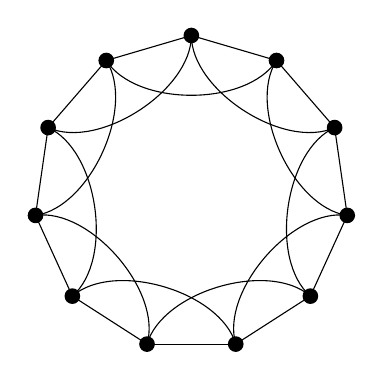
\begin{tikzpicture}
                  % Calculate positions for 11 nodes evenly distributed
                  % Draw edges: each node connects to adjacent nodes and nodes at distance 5
                  \foreach \i in {0,...,10} {
                    \pgfmathsetmacro{\next}{int(mod(\i+1,11))}
                    \pgfmathsetmacro{\jumptwo}{int(mod(\i+2,11))}
                    \draw ({90-\i*360/11}:2) -- ({90-\next*360/11}:2);
                    \draw ({90-\i*360/11}:2) .. controls ({90-\i*360/11}:1.3) and ({90-\jumptwo*360/11}:1.3) .. ({90-\jumptwo*360/11}:2);
                  }
                  
                  % Draw nodes on top
                  \foreach \i in {0,...,10} {
                    \node[circle, fill=black, inner sep=2pt] at ({90-\i*360/11}:2) {};
                  }
                \end{tikzpicture}
                \end{center}
          \item 22: een cyclus van 22 toppen, verbonden met 22 bogen
                \begin{center}
                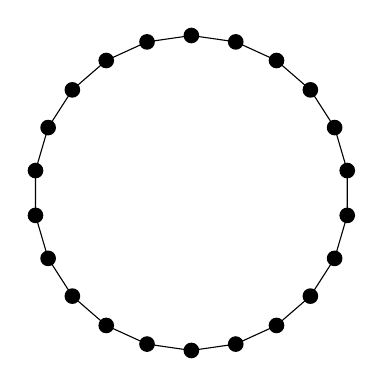
\begin{tikzpicture}
                  % Draw edges: each node connects to adjacent nodes
                  \foreach \i in {0,...,21} {
                    \pgfmathsetmacro{\next}{int(mod(\i+1,22))}
                    \draw ({90-\i*360/22}:2) -- ({90-\next*360/22}:2);
                  }
                  
                  % Draw nodes on top
                  \foreach \i in {0,...,21} {
                    \node[circle, fill=black, inner sep=2pt] at ({90-\i*360/22}:2) {};
                  }
                \end{tikzpicture}
                \end{center}
          \item \(\cancel{44}\): 44 toppen van graad 1 zou niet samenhangend zijn.
        \end{itemize}
\end{enumerate}

Als een graf met \(n\) toppen heeft van minstens graad \(\frac{n}{2}\), dan is het een Hamilotongraf.
Is er een top met een kleinere graad, dan weten we niks. Dan kan het nog steeds een Hamilotongraf zijn,
zoals \(C_{100}\): een cyclus van 100 toppen en 100 bogen heeft toppen van graad 2.

Een graf is \textbf{niet} Hamilton als er een top te vinden is die er voor zorgt dat, als je dit top
weg laat, de graf niet meer samenhangend is.

\begin{center}
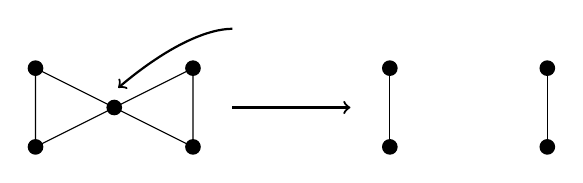
\begin{tikzpicture}

  \begin{scope}
    \draw (0,1) -- (1,0.5) -- (2,1) -- (2,0) -- (1,0.5) -- (0,0) -- cycle;
    
    \node[circle, fill=black, inner sep=2pt] (c1) at (0,1) {};
    \node[circle, fill=black, inner sep=2pt] (c2) at (1,0.5) {};
    \node[circle, fill=black, inner sep=2pt] (c3) at (2,1) {};
    \node[circle, fill=black, inner sep=2pt] (c4) at (2,0) {};
    \node[circle, fill=black, inner sep=2pt] (c5) at (0,0) {};
    
    % Arrow pointing to c2 from upper right
    \draw[->, thick] (2.5,1.5) .. controls (2.2,1.5) and (1.7,1.3) .. (1.05,0.75);
  \end{scope}

  \begin{scope}[xshift=2.5cm]
    % Arrow pointing right
    \draw[->, thick] (0,0.5) -- (1.5,0.5);
  \end{scope}

  \begin{scope}[xshift=4.5cm]
    \draw (0,1) -- (0,0);
    \draw (2,1) -- (2,0);
    
    \node[circle, fill=black, inner sep=2pt] (c1) at (0,1) {};
    \node[circle, fill=black, inner sep=2pt] (c3) at (2,1) {};
    \node[circle, fill=black, inner sep=2pt] (c4) at (2,0) {};
    \node[circle, fill=black, inner sep=2pt] (c5) at (0,0) {};
  \end{scope}

\end{tikzpicture}
\end{center}

Zo ook, als er 2 toppen te vinden zijn die er voor zorgen dat de graf in 3 of meer
componenten uit elkaar valt, is het geen Hamilton. Zie volgende figuur.

\begin{center}
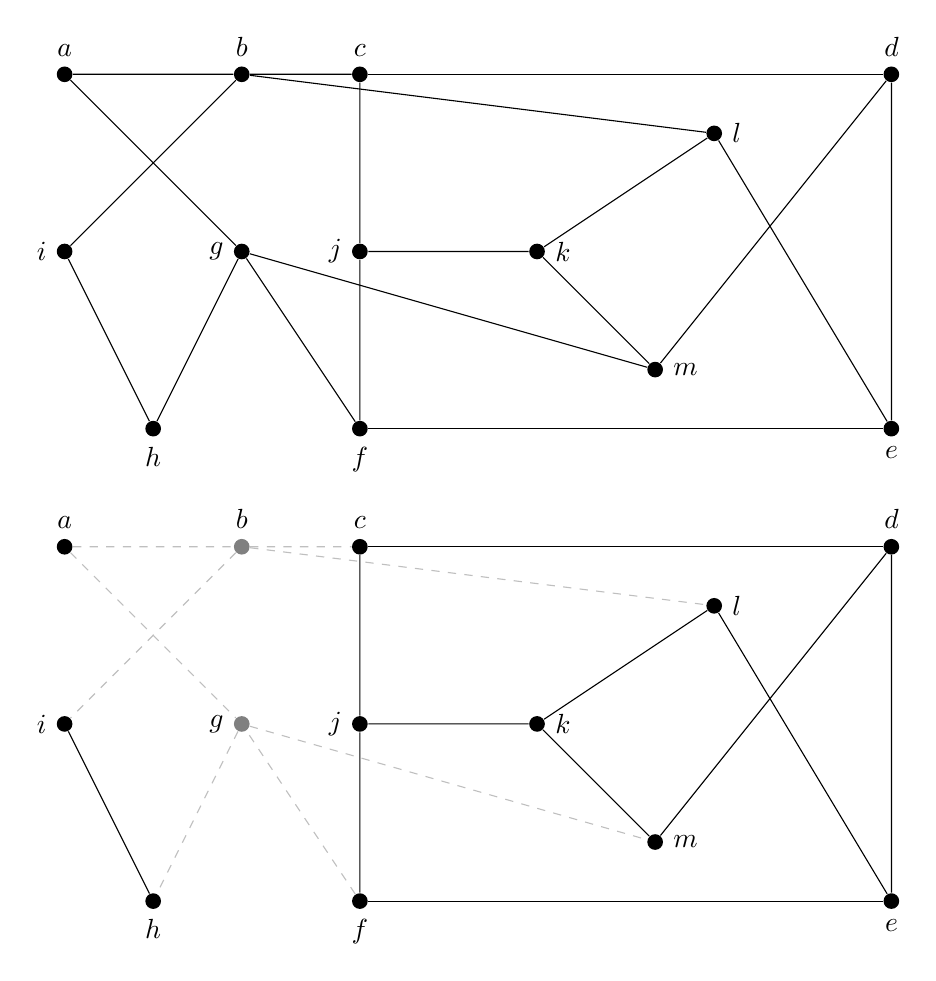
\begin{tikzpicture}[scale=1.5]
  \begin{scope}
    % Define node positions
    \node[circle, fill=black, inner sep=2pt, label=above:$a$] (a) at (0,3) {};
    \node[circle, fill=black, inner sep=2pt, label=above:$b$] (b) at (1.5,3) {};
    \node[circle, fill=black, inner sep=2pt, label=above:$c$] (c) at (2.5,3) {};
    \node[circle, fill=black, inner sep=2pt, label=above:$d$] (d) at (7,3) {};
    \node[circle, fill=black, inner sep=2pt, label=below:$e$] (e) at (7,0) {};
    \node[circle, fill=black, inner sep=2pt, label=below:$f$] (f) at (2.5,0) {};
    \node[circle, fill=black, inner sep=2pt, label=left :$g$] (g) at (1.5,1.5) {};
    \node[circle, fill=black, inner sep=2pt, label=below:$h$] (h) at (0.75,0) {};
    \node[circle, fill=black, inner sep=2pt, label=left :$i$] (i) at (0,1.5) {};
    \node[circle, fill=black, inner sep=2pt, label=left :$j$] (j) at (2.5,1.5) {};
    \node[circle, fill=black, inner sep=2pt, label=right:$k$] (k) at (4,1.5) {};
    \node[circle, fill=black, inner sep=2pt, label=right:$l$] (l) at (5.5,2.5) {};
    \node[circle, fill=black, inner sep=2pt, label=right:$m$] (m) at (5,0.5) {};
    
    % Draw edges
    \draw (a) -- (b);
    \draw (a) -- (g);
  s
    \draw (b) -- (c);
    \draw (b) -- (i);
    \draw (b) -- (l);

    \draw (c) -- (d);
    \draw (c) -- (j);

    \draw (d) -- (e);
    \draw (d) -- (m);

    \draw (e) -- (f);
    \draw (e) -- (l);

    \draw (f) -- (g);
    \draw (f) -- (j);

    \draw (g) -- (h);
    \draw (g) -- (m);

    \draw (h) -- (i);

    \draw (j) -- (k);

    \draw (k) -- (l);
    \draw (k) -- (m);
  \end{scope}

  \begin{scope}[yshift=-4cm]
    % Define node positions
    \node[circle, fill=black, inner sep=2pt, label=above:$a$] (a) at (0,3) {};
    \node[circle, fill=gray, inner sep=2pt, label=above:$b$] (b) at (1.5,3) {};
    \node[circle, fill=black, inner sep=2pt, label=above:$c$] (c) at (2.5,3) {};
    \node[circle, fill=black, inner sep=2pt, label=above:$d$] (d) at (7,3) {};
    \node[circle, fill=black, inner sep=2pt, label=below:$e$] (e) at (7,0) {};
    \node[circle, fill=black, inner sep=2pt, label=below:$f$] (f) at (2.5,0) {};
    \node[circle, fill=gray, inner sep=2pt, label=left :$g$] (g) at (1.5,1.5) {};
    \node[circle, fill=black, inner sep=2pt, label=below:$h$] (h) at (0.75,0) {};
    \node[circle, fill=black, inner sep=2pt, label=left :$i$] (i) at (0,1.5) {};
    \node[circle, fill=black, inner sep=2pt, label=left :$j$] (j) at (2.5,1.5) {};
    \node[circle, fill=black, inner sep=2pt, label=right:$k$] (k) at (4,1.5) {};
    \node[circle, fill=black, inner sep=2pt, label=right:$l$] (l) at (5.5,2.5) {};
    \node[circle, fill=black, inner sep=2pt, label=right:$m$] (m) at (5,0.5) {};
    
    % Draw edges
    \draw[gray!50, dashed] (a) -- (b);
    \draw[gray!50, dashed] (a) -- (g);
  s
    \draw[gray!50, dashed] (b) -- (c);
    \draw[gray!50, dashed] (b) -- (i);
    \draw[gray!50, dashed] (b) -- (l);

    \draw (c) -- (d);
    \draw (c) -- (j);

    \draw (d) -- (e);
    \draw (d) -- (m);

    \draw (e) -- (f);
    \draw (e) -- (l);

    \draw[gray!50, dashed] (f) -- (g);
    \draw (f) -- (j);

    \draw[gray!50, dashed] (g) -- (h);
    \draw[gray!50, dashed] (g) -- (m);

    \draw (h) -- (i);

    \draw (j) -- (k);

    \draw (k) -- (l);
    \draw (k) -- (m);
  \end{scope}

\end{tikzpicture}
\end{center}

\begin{enumerate}[start=25]
  \item Toon aan dat de Petersengraaf geen Hamiltoncyclus, maar wel een
        Hamiltonpad heeft. Toon aan dat, als je 1 top en de incidente bogen
        verwijdert uit de graf, er wel een Hamiltoncyclus is.

        \begin{center}
        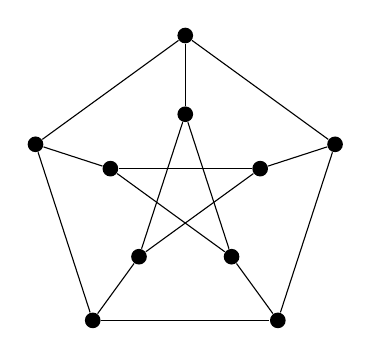
\begin{tikzpicture}[scale=2]
          \begin{scope}
            % Outer pentagon vertices
            \foreach \i in {0,...,4} {
              \node[circle, fill=black, inner sep=2pt] (outer\i) at ({90+\i*72}:1) {};
            }
            
            % Inner pentagon vertices (star pattern)
            \foreach \i in {0,...,4} {
              \node[circle, fill=black, inner sep=2pt] (inner\i) at ({90+\i*72}:0.5) {};
            }
            
            % Outer pentagon edges
            \foreach \i in {0,...,4} {
              \pgfmathsetmacro{\next}{int(mod(\i+1,5))}
              \draw (outer\i) -- (outer\next);
            }
            
            % Inner star edges (each vertex connects to vertex +2 mod 5)
            \foreach \i in {0,...,4} {
              \pgfmathsetmacro{\next}{int(mod(\i+2,5))}
              \draw (inner\i) -- (inner\next);
            }
            
            % Spokes connecting outer to inner
            \foreach \i in {0,...,4} {
              \draw (outer\i) -- (inner\i);
            }
          \end{scope}
        \end{tikzpicture}
        \end{center}

        Eigenschappen:
        \begin{itemize}
          \item elke top is 3-regulier
          \item het kortste pad heeft lengte 5
          \item 10 toppen
        \end{itemize}

        Bewering: er is geen graf die aan deze drie eigenschappen voldoet en een cyclus heeft.

        Als we een cyclus proberen te vervolledigen, komen we snel in de problemen.

        \begin{enumerate}
          \item De eerste rechte moet 4 toppen verder liggen, zodat er een lus van 5 gevormd wordt.
                De kleinste lus moet immers 5 zijn.
          \item Vanuit dat punt trekken we een nieuwe rechte naar 4 toppen verder. De twee rechten
                vormen samen met de tussenliggende top echter een nieuwe kortste lus van 4, wat
                niet mag.
        \end{enumerate}
        
        \begin{center}
        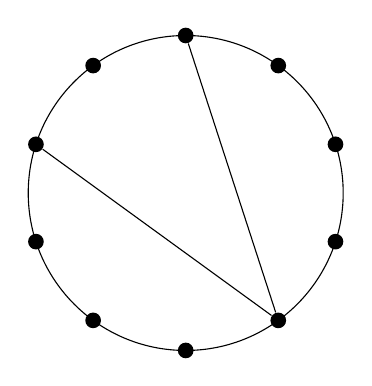
\begin{tikzpicture}[scale=2]
          \begin{scope}[xshift=3cm]
            % Draw the circle
            \draw (0,0) circle (1);
            
            % 10 nodes evenly distributed on a circle
            \foreach \i in {0,...,9} {
              \node[circle, fill=black, inner sep=2pt] (n\i) at ({90-\i*36}:1) {};
            }

            \draw (n0) -- (n4);
            \draw (n4) -- (n8);
          \end{scope}
        \end{tikzpicture}
        \end{center}
         
        \begin{center}
        \begin{tikzpicture}[scale=2]
            \begin{scope}
            % Outer pentagon vertices
            \foreach \i in {0,...,4} {
              \node[circle, fill=black, inner sep=2pt] (outer\i) at ({90+\i*72}:1) {};
            }
            
            % Inner pentagon vertices (star pattern)
            \foreach \i in {0,...,4} {
              \node[circle, fill=black, inner sep=2pt] (inner\i) at ({90+\i*72}:0.5) {};
            }
            
            % Outer pentagon edges
            \foreach \i in {0,...,4} {
              \pgfmathsetmacro{\next}{int(mod(\i+1,5))}
              \draw (outer\i) -- (outer\next);
            }
            
            % Inner star edges (each vertex connects to vertex +2 mod 5)
            \foreach \i in {0,...,4} {
              \pgfmathsetmacro{\next}{int(mod(\i+2,5))}
              \draw (inner\i) -- (inner\next);
            }
            
            % Spokes connecting outer to inner
            \foreach \i in {0,...,4} {
              \draw (outer\i) -- (inner\i);
            }

            \draw[pad-pijl] (outer0) -- (outer1);
            \draw[pad-pijl] (outer1) -- (outer2);
            \draw[pad-pijl] (outer2) -- (outer3);
            \draw[pad-pijl] (outer3) -- (outer4);
            \draw[pad-pijl] (outer4) -- (inner4);
            \draw[pad-pijl] (inner4) -- (inner2);
            \draw[pad-pijl] (inner2) -- (inner0);
            \draw[pad-pijl] (inner0) -- (inner3);
            \draw[pad-pijl] (inner3) -- (inner1);
          \end{scope}

          \begin{scope}[xshift=2.5cm]
            % Outer pentagon vertices
            \foreach \i in {1,...,4} {
              \node[circle, fill=black, inner sep=2pt] (outer\i) at ({90+\i*72}:1) {};
            }
            
            % Inner pentagon vertices (star pattern)
            \foreach \i in {0,...,4} {
              \node[circle, fill=black, inner sep=2pt] (inner\i) at ({90+\i*72}:0.5) {};
            }
            
            % Outer pentagon edges
            \foreach \i in {1,...,3} {
              \pgfmathsetmacro{\next}{int(mod(\i+1,5))}
              \draw (outer\i) -- (outer\next);
            }
            
            % Inner star edges (each vertex connects to vertex +2 mod 5)
            \foreach \i in {0,...,4} {
              \pgfmathsetmacro{\next}{int(mod(\i+2,5))}
              \draw (inner\i) -- (inner\next);
            }
            
            % Spokes connecting outer to inner
            \foreach \i in {1,...,4} {
              \draw (outer\i) -- (inner\i);
            }

            % removed
            \node[circle, fill=gray!50, inner sep=2pt] (outer0) at (90:1) {};
            \draw[gray!50] (outer0) -- (outer1);
            \draw[gray!50] (outer0) -- (outer4);
            \draw[gray!50] (outer0) -- (inner0);

            
            \draw[pad-pijl] (outer1) -- (outer2);
            \draw[pad-pijl] (outer2) -- (outer3);
            \draw[pad-pijl] (outer3) -- (outer4);
            \draw[pad-pijl] (outer4) -- (inner4);
            \draw[pad-pijl] (inner4) -- (inner2);
            \draw[pad-pijl] (inner2) -- (inner0);
            \draw[pad-pijl] (inner0) -- (inner3);
            \draw[pad-pijl] (inner3) -- (inner1);
            \draw[pad-pijl] (inner1) -- (outer1);
          \end{scope}

          \begin{scope}[xshift=5cm]
            % Outer pentagon vertices
            \foreach \i in {0,...,4} {
              \node[circle, fill=black, inner sep=2pt] (outer\i) at ({90+\i*72}:1) {};
            }
            
            % Inner pentagon vertices (star pattern)
            \foreach \i in {1,...,4} {
              \node[circle, fill=black, inner sep=2pt] (inner\i) at ({90+\i*72}:0.5) {};
            }
            
            \node[circle, fill=gray!50, inner sep=2pt] (inner0) at (90:0.5) {};

            % Outer pentagon edges
            \foreach \i in {0,...,4} {
              \pgfmathsetmacro{\next}{int(mod(\i+1,5))}
              \draw (outer\i) -- (outer\next);
            }
            
            % Inner star edges (each vertex connects to vertex +2 mod 5)
            \foreach \i in {1,2,4} {
              \pgfmathsetmacro{\next}{int(mod(\i+2,5))}
              \draw (inner\i) -- (inner\next);
            }
            
            % Spokes connecting outer to inner
            \foreach \i in {1,...,4} {
              \draw (outer\i) -- (inner\i);
            }

            % removed
            \draw[gray!50] (outer0) -- (inner0);
            \draw[gray!50] (inner0) -- (inner2);
            \draw[gray!50] (inner0) -- (inner3);

            
            \draw[pad-pijl] (inner2) -- (inner4);
            \draw[pad-pijl] (inner4) -- (inner1);
            \draw[pad-pijl] (inner1) -- (inner3);
            \draw[pad-pijl] (inner3) -- (outer3);
            \draw[pad-pijl] (outer3) -- (outer4);
            \draw[pad-pijl] (outer4) -- (outer0);
            \draw[pad-pijl] (outer0) -- (outer1);
            \draw[pad-pijl] (outer1) -- (outer2);
            \draw[pad-pijl] (outer2) -- (inner2);
          \end{scope}
        \end{tikzpicture}
        \end{center}

        
        In de linker figuur, hebben we een open Hamiltonpad. Door 1 top te verwijderen,
        hebben we een gesloten pad, en dus een Hamiltoncyclus.
\end{enumerate}

\begin{tcolorbox}[title=Ter herinnering]
  Bij bomen:
  \[ |E(\mathcal{G})| = |V(\mathcal{G})| - 1\]
\end{tcolorbox}

\begin{enumerate}[start=29]
  \item Teken alle niet-isomorfe bomen met zes toppen
        \begin{center}
          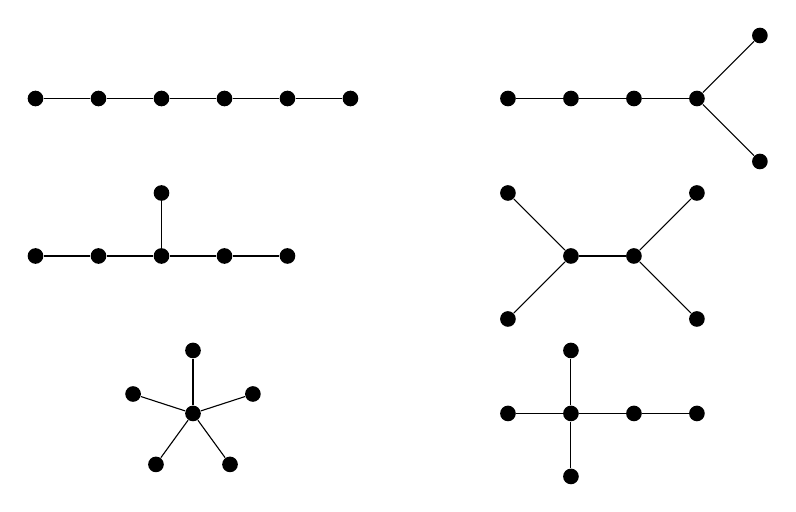
\begin{tikzpicture}
            % Tree 1: Path graph (6 nodes in a line)
            \begin{scope}[xshift=0cm]
              \foreach \i in {0,...,5} {
                \node[circle, fill=black, inner sep=2pt] (n\i) at (\i*0.8,0) {};
              }
              \foreach \i in {0,...,4} {
                \pgfmathsetmacro{\next}{int(\i+1)}
                \draw (n\i) -- (n\next);
              }
            \end{scope}

            % Tree 2: Path with one branch at end
            \begin{scope}[xshift=6cm]
              \foreach \i in {0,...,3} {
                \node[circle, fill=black, inner sep=2pt] (n\i) at (\i*0.8,0) {};
              }
              \node[circle, fill=black, inner sep=2pt] (n4) at (3.2, 0.8) {};
              \node[circle, fill=black, inner sep=2pt] (n5) at (3.2,-0.8) {};
              
              \foreach \i in {0,...,2} {
                \pgfmathsetmacro{\next}{int(\i+1)}
                \draw (n\i) -- (n\next);
              }
              \draw (n3) -- (n4);
              \draw (n3) -- (n5);
            \end{scope}

            % Tree 3: Path with branch in middle
            \begin{scope}[yshift=-2cm, xshift=0cm]
              \foreach \i in {0,...,4} {
                \node[circle, fill=black, inner sep=2pt] (n\i) at (\i*0.8,0) {};
              }
              \node[circle, fill=black, inner sep=2pt] (n5) at (1.6,0.8) {};
              
              \foreach \i in {0,...,3} {
                \pgfmathsetmacro{\next}{int(\i+1)}
                \draw (n\i) -- (n\next);
              }
              \draw (n2) -- (n5);
            \end{scope}

            % Tree 4: Y-shape (one node with 3 branches)
            \begin{scope}[yshift=-2cm, xshift=6cm]
              \node[circle, fill=black, inner sep=2pt] (n1) at (0,-0.8) {};
              \node[circle, fill=black, inner sep=2pt] (n2) at (0, 0.8) {};
              \node[circle, fill=black, inner sep=2pt] (n3) at (0.8,0) {};
              \node[circle, fill=black, inner sep=2pt] (n4) at (1.6,0) {};
              \node[circle, fill=black, inner sep=2pt] (n5) at (2.4,-0.8) {};
              \node[circle, fill=black, inner sep=2pt] (n6) at (2.4,0.8) {};
              
              \draw (n1) -- (n3);
              \draw (n2) -- (n3);
              \draw (n3) -- (n4);
              \draw (n4) -- (n5);
              \draw (n4) -- (n6);
            \end{scope}

            % Tree 5: Star graph (one center with 5 branches)
            \begin{scope}[yshift=-4cm, xshift=2cm]
              \node[circle, fill=black, inner sep=2pt] (center) at (0,0) {};
              \foreach \i in {0,...,4} {
                \node[circle, fill=black, inner sep=2pt] (n\i) at ({90+\i*72}:0.8) {};
                \draw (center) -- (n\i);
              }
            \end{scope}

            % Tree 6: Cross graph
            \begin{scope}[yshift=-4cm, xshift=6cm]
              \foreach \i in {0,...,3} {
                \node[circle, fill=black, inner sep=2pt] (n\i) at (\i*0.8,0) {};
              }
              \node[circle, fill=black, inner sep=2pt] (n4) at (0.8,-0.8) {};
              \node[circle, fill=black, inner sep=2pt] (n5) at (0.8, 0.8) {};
              
              \foreach \i in {0,...,2} {
                \pgfmathsetmacro{\next}{int(\i+1)}
                \draw (n\i) -- (n\next);
              }
              \draw (n1) -- (n4);
              \draw (n1) -- (n5);

            \end{scope}
          \end{tikzpicture}
        \end{center}
\end{enumerate}

\begin{enumerate}[start=34]
  \item Zoek 2 niet-isomorfe opspannende bomen voor de complete bipartiete
        graaf \(K_{2,3}\). Hoeveel niet-isomorfe opspannende bomen heeft deze graf?

        \begin{figure}[H]
          \centering
          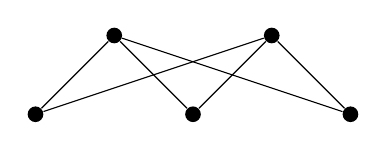
\begin{tikzpicture}
            \begin{scope}[xshift=0cm]
              \node[circle, fill=black, inner sep=2pt] (n0) at (0,0) {};
              \node[circle, fill=black, inner sep=2pt] (n1) at (1,1) {};
              \node[circle, fill=black, inner sep=2pt] (n2) at (2,0) {};
              \node[circle, fill=black, inner sep=2pt] (n3) at (3,1) {};
              \node[circle, fill=black, inner sep=2pt] (n4) at (4,0) {};
              
              \draw (n0) -- (n1);
              \draw (n0) -- (n3);
              \draw (n2) -- (n1);
              \draw (n2) -- (n3);
              \draw (n4) -- (n1);
              \draw (n4) -- (n3);
            \end{scope}
          \end{tikzpicture}
          \caption{\(K_{2,3}\)}
        \end{figure}

        We mogen enkel bogen weglaten, geen toppen.

        \begin{figure}[H]
          \centering
          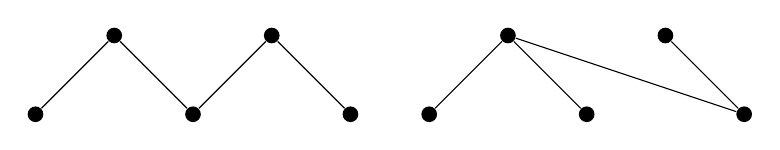
\begin{tikzpicture}
            \begin{scope}[xshift=0cm]
              \node[circle, fill=black, inner sep=2pt] (n0) at (0,0) {};
              \node[circle, fill=black, inner sep=2pt] (n1) at (1,1) {};
              \node[circle, fill=black, inner sep=2pt] (n2) at (2,0) {};
              \node[circle, fill=black, inner sep=2pt] (n3) at (3,1) {};
              \node[circle, fill=black, inner sep=2pt] (n4) at (4,0) {};
              
              \draw (n0) -- (n1);
              \draw (n2) -- (n1);
              \draw (n2) -- (n3);
              \draw (n4) -- (n3);
            \end{scope}
            
            \begin{scope}[xshift=5cm]
              \node[circle, fill=black, inner sep=2pt] (n0) at (0,0) {};
              \node[circle, fill=black, inner sep=2pt] (n1) at (1,1) {};
              \node[circle, fill=black, inner sep=2pt] (n2) at (2,0) {};
              \node[circle, fill=black, inner sep=2pt] (n3) at (3,1) {};
              \node[circle, fill=black, inner sep=2pt] (n4) at (4,0) {};
              
              \draw (n0) -- (n1);
              \draw (n2) -- (n1);
              \draw (n4) -- (n1);
              \draw (n4) -- (n3);
            \end{scope}
          \end{tikzpicture}
        \end{figure}
  
  % Oefening 35
  \item Zoek alle maximale koppelingen van de Petersengraaf. Hoe groot is
        een maximumkoppeling van deze graf?

        \begin{center}
        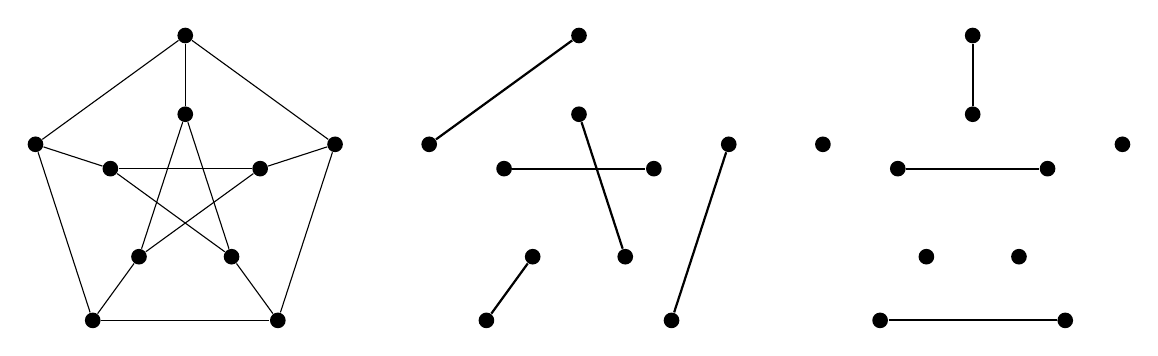
\begin{tikzpicture}[scale=2]
          \begin{scope}
            % Outer pentagon vertices
            \foreach \i in {0,...,4} {
              \node[circle, fill=black, inner sep=2pt] (outer\i) at ({90+\i*72}:1) {};
            }
            
            % Inner pentagon vertices (star pattern)
            \foreach \i in {0,...,4} {
              \node[circle, fill=black, inner sep=2pt] (inner\i) at ({90+\i*72}:0.5) {};
            }
            
            % Outer pentagon edges
            \foreach \i in {0,...,4} {
              \pgfmathsetmacro{\next}{int(mod(\i+1,5))}
              \draw (outer\i) -- (outer\next);
            }
            
            % Inner star edges (each vertex connects to vertex +2 mod 5)
            \foreach \i in {0,...,4} {
              \pgfmathsetmacro{\next}{int(mod(\i+2,5))}
              \draw (inner\i) -- (inner\next);
            }
            
            % Spokes connecting outer to inner
            \foreach \i in {0,...,4} {
              \draw (outer\i) -- (inner\i);
            }
          \end{scope}
          
          \begin{scope}[xshift=2.5cm]
            % Outer pentagon vertices
            \foreach \i in {0,...,4} {
              \node[circle, fill=black, inner sep=2pt] (outer\i) at ({90+\i*72}:1) {};
            }
            
            % Inner pentagon vertices (star pattern)
            \foreach \i in {0,...,4} {
              \node[circle, fill=black, inner sep=2pt] (inner\i) at ({90+\i*72}:0.5) {};
            }
            

            \draw[thick] (outer0) -- (outer1);
            \draw[thick] (outer3) -- (outer4);
            \draw[thick] (outer2) -- (inner2);
            \draw[thick] (inner0) -- (inner3);
            \draw[thick] (inner1) -- (inner4);
          \end{scope}
          
          \begin{scope}[xshift=5cm]
            % Outer pentagon vertices
            \foreach \i in {0,...,4} {
              \node[circle, fill=black, inner sep=2pt] (outer\i) at ({90+\i*72}:1) {};
            }
            
            % Inner pentagon vertices (star pattern)
            \foreach \i in {0,...,4} {
              \node[circle, fill=black, inner sep=2pt] (inner\i) at ({90+\i*72}:0.5) {};
            }
            
            \draw[thick] (outer0) -- (inner0);
            \draw[thick] (outer2) -- (outer3);
            \draw[thick] (inner1) -- (inner4);
          \end{scope}
        \end{tikzpicture}
        \end{center}
        
        De maximumgrootte is 5.
\end{enumerate}

\begin{tcolorbox}[title=Ter herinnering]
  Wat is een eindige 2-reguliere graf?
  
  Elke cyclus geeft ons een eindige 2-reguliere graf.   Niet elke 2-reguliere graf is een cyclus, bvb. een gaf bestaande uit meerdere samenhangscomponenten.

  Een eindige 2-reguliere graf is een graf waarin elke samenhangscomponent een cyclus is.
\end{tcolorbox}

\begin{enumerate}[start=37]
  % Oefening 37
  \item Aan een toernooi doen \(2n\) ploegen mee. Er zijn al twee ronden
        gespeeld. Toon aan dat we de ploegen nog altijd in twee groepen van
        \(n\) ploegen kunnen verdelen, zodat ploegen van eenzelfde groep nog niet
        tegen elkaar gespeeld hebben.

        \(\mathcal{G}\):

        \(V(\mathcal{G}) = \) \{ploegen\}

        \(E(\mathcal{G}) = \{p \sim q \mid p, q \in V(\mathcal{G})\) zodat \(p\) reeds tegen \(q\)
        gespeeld heeft \(\}\)

        \(\mathcal{G}\) is 2-regulier, aangezien elke ploeg 2 wedstrijden heeft gespeeld. Alle 
        samenhangscomponenten van \(\mathcal{G}\) zijn dus cycli.

        \begin{center}
        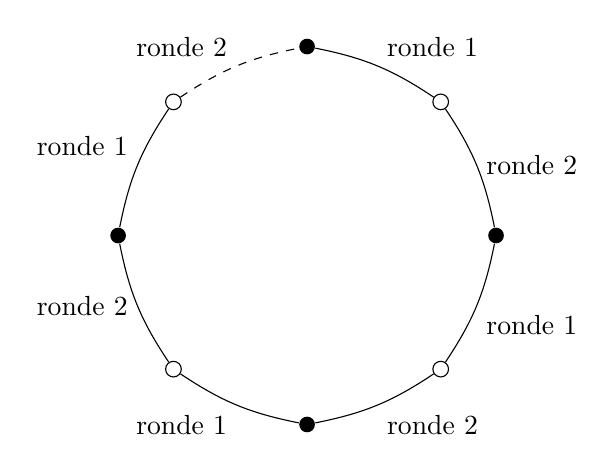
\begin{tikzpicture}[scale=1.2]
          % Define the nodes in a circular pattern
          \node[circle, fill=black, inner sep=2pt] (n1) at (90:2) {};
          \node[circle, draw=black, inner sep=2pt] (n2) at (45:2) {};
          \node[circle, fill=black, inner sep=2pt] (n3) at (0:2) {};
          \node[circle, draw=black, inner sep=2pt] (n4) at (-45:2) {};
          \node[circle, fill=black, inner sep=2pt] (n5) at (-90:2) {};
          \node[circle, draw=black, inner sep=2pt] (n6) at (-135:2) {};
          \node[circle, fill=black, inner sep=2pt] (n7) at (180:2) {};
          \node[circle, draw=black, inner sep=2pt] (n8) at (135:2) {};
          
          % Draw edges forming the cycle with bends to create a perfect circle
          \draw (n1) to[bend left=11.25] node[midway, above right] {ronde 1} (n2);
          \draw (n2) to[bend left=11.25] node[midway, right] {ronde 2} (n3);
          \draw (n3) to[bend left=11.25] node[midway, below right] {ronde 1} (n4) ;
          \draw (n4) to[bend left=11.25] node[midway, below right] {ronde 2} (n5) ;
          \draw (n5) to[bend left=11.25] node[midway, below left] {ronde 1} (n6) ;
          \draw (n6) to[bend left=11.25] node[midway, left] {ronde 2} (n7) ;
          \draw (n7) to[bend left=11.25] node[midway, above left] {ronde 1} (n8) ;
          
          % Dashed edge
          \draw[dashed] (n8) to[bend left=11.25] node[midway, above left] {ronde 2} (n1);
        \end{tikzpicture}
        \end{center}

        Alle samenhangscomponenten moeten een even aantal toppen hebben. Anders zou er 
        een ploeg zijn die twee keer in dezelfde ronde heeft gespeeld, wat niet kan.

        We kunnen de toppen dus alternerend aan een groep toevoegen. Deze ploegen hebben
        dan niet tegen elkaar gespeeld.
  
  % Oefening 38
  \item Zij \((X \cup Y, \sim)\) een bipartiete graaf waarin de graad van elke top in
        \(X\) minstens zo groot is als de graad van elke top in \(Y\). Toon aan dat
        er een toewijzing bestaat van \(X\) in \(Y\).

        \(\deg(x) \geq \deg(y) \qquad \forall x \in X, y \in Y \)

        \(m = \min \deg(x), x \in X \qquad\qquad M = \max \deg(y), y \in Y\)

        \(m \geq M\)

        \(W \subset X \) willekeurig

        \textbf{Te bewijzen:} \(|H(W)| \geq |W|\)

        \textbf{Bewijs:}
        \begin{align*}
          \begin{array}{ccccccc}
            \displaystyle
            \sum_{x \in W} m & \leq & \displaystyle \sum_{x \in W} \deg(x) & \leq & \displaystyle \sum_{y \in H(W)} \deg (j) & \leq & \displaystyle \sum_{y \in H(W)} M \\
            \|               &      &                        &                    &                            &      &  \|       \\
            m |W|            &      &                        &                   &                            &      & M |H(W)| \\
          \end{array}
        \end{align*}

        \(\Rightarrow m |W| \leq M |H(W)|\)
        \(\Rightarrow |W| \leq \frac{M}{m} |H(W)| \leq 1 \cdot |H(W)| = |H(W)|\)
\end{enumerate}

\begin{tcolorbox}[title=Ter herinnering]
  \((X \cup Y, \sim)\) is een bipartiete graf. Toppen van \(X\) zijn niet met elkaar
  verbonden. Toppen van \(Y\) zijn niet met elkaar verbonden. \quad \(W \subset X\).

  Een toewijzing van \(W\) is een koppeling die \(W\) verzadigt.
  \\[1em]
  \textbf{Hall}: er bestaat een toewijzing van \(W\) als en slechts als 
  \[ \forall W' \subset W: |H(W')| \geq |W'|\]

  \(H(W')\) zijn de buren van \(W'\)
\end{tcolorbox}

\begin{enumerate}[start=45]
  % Oefening 45
  \item Fritz moet jobs toewijzen aan jobstudenten. Hij heeft 25 kandidaten
        en 25 jobs die moeten ingevuld worden. Elke student is voor minstens
        4 jobs geschikt, maar elke job kan door ten hoogste 4 studenten uitgevoerd
        worden. Kan Fritz elke student een job geven waarvoor hij geschikt is? Leg uit.

        \((S \cup J, \sim)\) \qquad \(W \subset S\) willekeurig

        \textbf{Te bewijzen:} \(|H(W)| \geq |W|\)

        \textbf{Bewijs:}
        \begin{align*}
          \begin{array}{ccccccc}
            \displaystyle
            \sum_{s \in W} 4 & \leq & \displaystyle \sum_{s \in W} \deg(s) & \stackrel{?}{\leq} & \displaystyle \sum_{j \in H(W)} \deg (j) & \leq & \displaystyle \sum_{j \in H(W)} 4 \\
            \|               &      &                        &                    &                            &      &  \|       \\
            4 |W|            &      &                        &                   &                            &      & 4 |H(W)| \\
            \sum_{s \in W} 4 & \leq & \displaystyle \sum_{s \in W} \deg(s) & \stackrel{!}{\leq} & \displaystyle \sum_{j \in H(W)} \deg (j) & \leq & \displaystyle \sum_{j \in H(W)} 4 \\
          \end{array}
        \end{align*}

        \( \sum_{s \in W} \deg(s)\): gaat uit \(S\) \textit{vertrekkende} bogen tellen.
        Aangezien er tussen toppen uit \(S\) onderling geen bogen gaan, worden deze bogen
        dus niet dubbel geteld.

        \(\sum_{j \in H(W)} \deg (j)\): telt de uit \(H(W)\) vertrekkende bogen.

        Elke boog die vertrekt uit \(W\), komt toe in \(H(W)\), dus \( \sum_{s \in W} \deg(s) \leq \sum_{j \in H(W)} \deg (j)\)

        \(\Rightarrow 4 |W| \leq 4 |H(W)|\) \\
        \(\Rightarrow |W| \leq |H(W)|\)

        De voorwaarde van de stelling van Hall is bewezen, dus we mogen er van uit gaan 
        dat er een toewijzing bestaat.

\end{enumerate}

\begin{tcolorbox}[title=Methode 1 om planaire graffen te herkennen]
  De \(K_5\) en \(K_{3,3}\) graffen:

  \begin{center}
    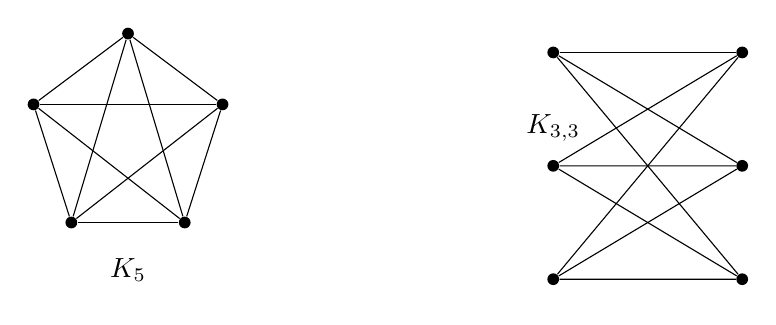
\begin{tikzpicture}[scale=1.2, every node/.style={circle, fill=black, inner sep=1.5pt}]
      \begin{scope}
        \node[draw=none,fill=none] at (0,-0.5) {$K_5$};

        \node (c1) at (0,2) {};
        \node (c2) at (-1,1.25) {};
        \node (c3) at ( 1,1.25) {};
        \node (c4) at (-0.60, 0) {};
        \node (c5) at ( 0.60, 0) {};
        
        \foreach \i in {1,...,5} {
          \foreach \j in {1,...,5} {
            \ifnum\i<\j
              \draw (c\i)--(c\j);
            \fi
          }
        }
      \end{scope}

      \begin{scope}[xshift=4.5cm,yshift=1cm]
        \node[draw=none,fill=none] at (0,0) {$K_{3,3}$};

        \foreach \i in {1,2,3} {
          \node (a\i) at (0,2-1.2*\i) {};
          \node (b\i) at (2,2-1.2*\i) {};
        }
        \foreach \i in {1,2,3} {
          \foreach \j in {1,2,3} {
            \draw (a\i)--(b\j);
          }
        }
      \end{scope}
    \end{tikzpicture}
  \end{center}
  \(\deg K_5 = 4 \qquad \deg K_{3,3} = 3\)

  Wat is de graad van de toppen? Zou er een \(K_5\) of een \(K_{3,3}\) te vinden kunnen zijn?
\end{tcolorbox}

\begin{enumerate}[start=50]
  \item Bepaal welke van de volgende grafen planair is. Teken de planaire
        grafen zonder dat de bogen snijden. Zoek in de grafen die niet planair
        zijn een deelgraaf die boogequivalent is met \(K_5\) of \(K_{3,3}\).

        \begin{enumerate}[label=\arabic*]
          \item niet-planair: we kunnen de toppen van graad 2 vervangen door een boog. Deze wordt dan \(K_{3,3}\)
          \item planair
          \item de toppen hebben graad 3, zoals bij \(K_{3,3}\). \(K_{5}\) heeft toppen van graad 4 en kunnen we
                dus niet krijgen door boogequivalentieoperaties.

                Als we één top met bijhorende bogen weglaten, wordt de graad van de aangrenzende toppen 2 en 
                houden we dus maar 4 toppen van graad 3 over. \(K_{3,3}\) heeft 6 toppen van graad 3.

                Als we één boog weglaten, krijgen we 2 toppen van graad 2. Als we vervolgens deze weglaten, 
                houden we \(K_{3,3}\) over.
          \item planair
          \item planair
          \item Deze top heeft 5 toppen met graad minstens 4. Hier vinden we waarschijnlijk een \(_5\).
        \end{enumerate}

        \begin{center}
          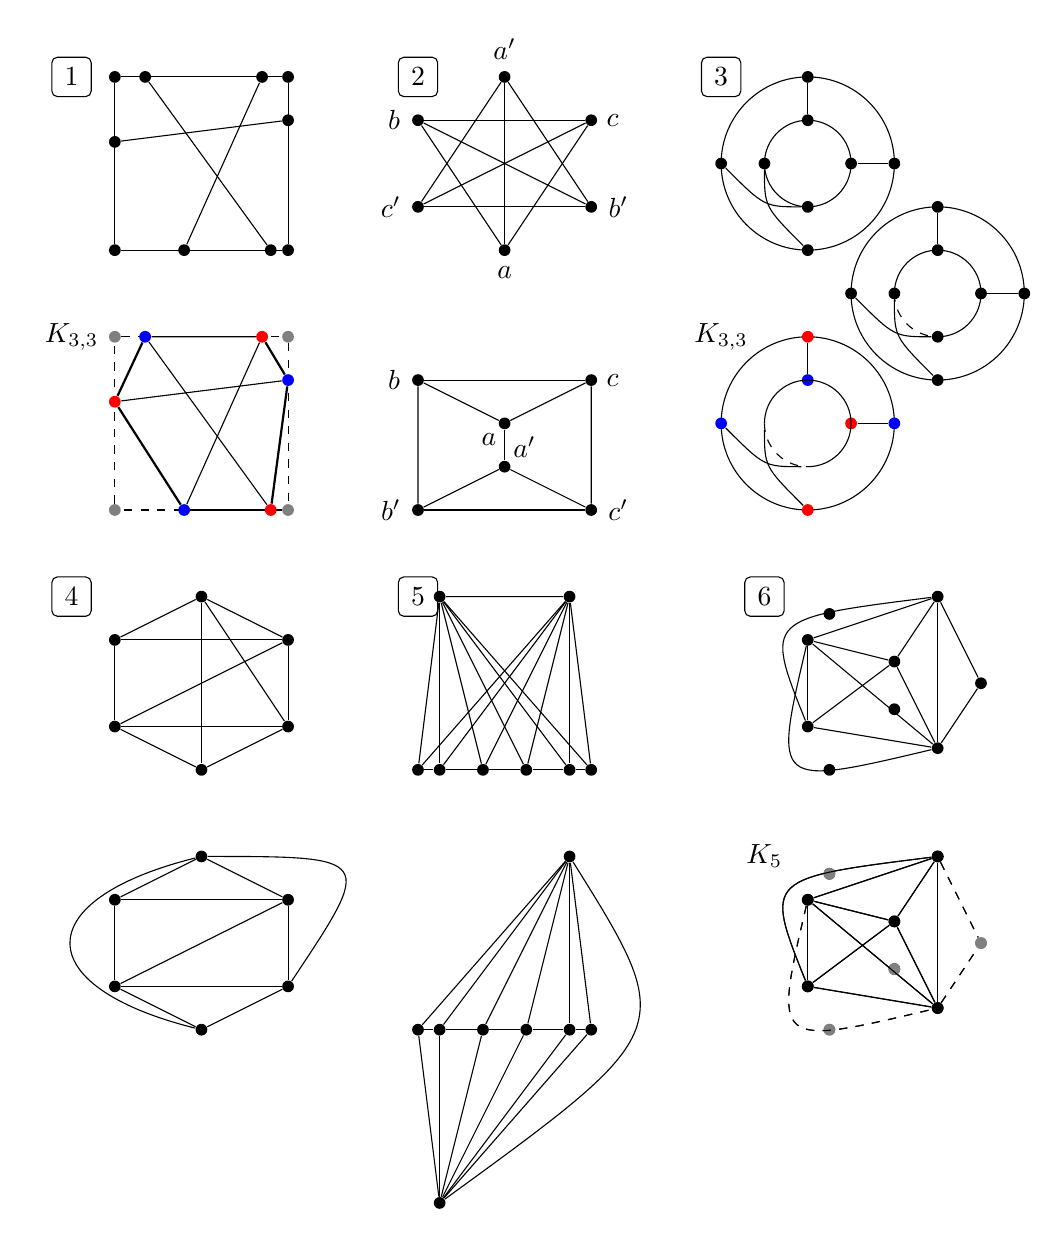
\begin{tikzpicture}[scale=1.1, every node/.style={circle, fill=black, inner sep=1.5pt}]

            \begin{scope}
              \node[draw, rectangle, rounded corners=2pt, minimum width=0.5cm, minimum height=0.5cm, fill=white] at (-0.5,2) {1};
              \node (a1)  at (0, 0) {};
              \node (a2)  at (0, 2) {};
              \node (a3)  at (2, 2) {};
              \node (a4)  at (2, 0) {};
              \draw (a1)  -- (a2) -- (a3) -- (a4) -- (a1);
              
              \node (a5)  at (0, 1.25) {};
              \node (a6)  at (2, 1.50) {};
              \draw (a5)  -- (a6);
              
              \node (a7)  at (0.35, 2) {};
              \node (a8)  at (1.80, 0) {};
              \draw (a7)  -- (a8);
              
              \node (a9)  at (1.7, 2) {};
              \node (a10) at (0.8, 0) {};
              \draw (a9) -- (a10);
            \end{scope}
            
            \begin{scope}[yshift=-3cm]
              \node[draw=none, fill=none, inner sep=0pt] at (-0.5,2) {\(K_{3,3}\)};
              \node[fill=gray] (a1)  at (0, 0) {};
              \node[fill=gray] (a2)  at (0, 2) {};
              \node[fill=gray] (a3)  at (2, 2) {};
              \node[fill=gray] (a4)  at (2, 0) {};
              \draw[dashed] (a1)  -- (a2) -- (a3) -- (a4) -- (a1);
              
              \node[fill=red] (a5)  at (0, 1.25) {};
              \node[fill=blue] (a6)  at (2, 1.50) {};
              
              \node[fill=blue] (a7)  at (0.35, 2) {};
              \node[fill=red] (a8)  at (1.80, 0) {};
              \draw (a5)  -- (a6);
              \draw (a7)  -- (a8);
              
              \node[fill=red] (a9)  at (1.7, 2) {};
              \node[fill=blue] (a10) at (0.8, 0) {};
              \draw (a7) -- (a9);
              \draw (a9) -- (a10);
              \draw (a8) -- (a10);

              \draw[thick] (a5)  -- (a7);
              \draw[thick] (a9)  -- (a6);
              \draw[thick] (a6)  -- (a8);
              \draw[thick] (a5)  -- (a10);
            \end{scope}

            \begin{scope}[xshift=4.5cm]
              \node[draw, rectangle, rounded corners=2pt, minimum width=0.5cm, minimum height=0.5cm, fill=white] at (-1,2) {2};
              \node[label=below:$a$ ] (b1)  at ( 0   , 0) {};
              \node[label=left :$c'$] (b2)  at (-1. , 0.5) {};
              \node[label=right:$b'$] (b3)  at ( 1. , 0.5) {};
              \node[label=left :$b$ ] (b4)  at (-1., 1.50) {};
              \node[label=right:$c$ ] (b5)  at ( 1., 1.50) {};
              \node[label=above:$a'$] (b6)  at ( 0   , 2) {};

              \draw (b1)  -- (b4);
              \draw (b1)  -- (b5);
              \draw (b1)  -- (b6);

              \draw (b2)  -- (b3);
              \draw (b2)  -- (b5);
              \draw (b2)  -- (b6);

              \draw (b3)  -- (b4);
              \draw (b3)  -- (b6);

              \draw (b4)  -- (b5);
            \end{scope}

            \begin{scope}[xshift=4.5cm,yshift=-3cm]
              \node[label=below left:$a$ ] (b1)  at ( 0  , 1) {};
              \node[label=right:$c'$] (b2)  at ( 1  , 0) {};
              \node[label=left :$b'$] (b3)  at (-1  , 0) {};
              \node[label=left :$b$ ] (b4)  at (-1  , 1.50) {};
              \node[label=right:$c$ ] (b5)  at ( 1  , 1.50) {};
              \node[label=above right:$a'$] (b6)  at ( 0 , 0.50) {};

              \draw (b1)  -- (b4);
              \draw (b1)  -- (b5);
              \draw (b1)  -- (b6);

              \draw (b2)  -- (b3);
              \draw (b2)  -- (b5);
              \draw (b2)  -- (b6);

              \draw (b3)  -- (b4);
              \draw (b3)  -- (b6);

              \draw (b4)  -- (b5);
            \end{scope}

            \begin{scope}[xshift=8cm,yshift=1cm]
              \node[draw, rectangle, rounded corners=2pt, minimum width=0.5cm, minimum height=0.5cm, fill=white] at (-1,1) {3};
              \draw (0,0) circle [radius=0.5cm];
              \draw (0,0) circle [radius=1cm];

              \node (c1)  at (-0.5, 0) {};
              \node (c2)  at ( 0  , 0.5) {};
              \node (c3)  at ( 0.5 , 0) {};
              \node (c4)  at ( 0. ,-0.5) {};

              \node (c5)  at ( -1, 0) {};
              \node (c6)  at ( 0   , 1) {};
              \node (c7)  at ( 1   , 0) {};
              \node (c8)  at ( 0   , -1) {};

              \draw (c2)  -- (c6);
              \draw (c3)  -- (c7);
              \draw (c1)  .. controls(-0.5, -0.5) .. (c8);
              \draw (c4)  .. controls(-0.5, -0.5) .. (c5);
            \end{scope}

            \begin{scope}[xshift=9.5cm,yshift=-0.5cm]
              % \draw (0,0) circle [radius=0.5cm];
              \draw (0,0) circle [radius=1cm];
              
              \node (c1)  at (-0.5, 0) {};
              \node (c2)  at ( 0  , 0.5) {};
              \node (c3)  at ( 0.5 , 0) {};
              \node (c4)  at ( 0. ,-0.5) {};
              
              \node (c5)  at ( -1, 0) {};
              \node (c6)  at ( 0   , 1) {};
              \node (c7)  at ( 1   , 0) {};
              \node (c8)  at ( 0   , -1) {};

              \draw (c4) arc[start angle=-90, end angle=180, radius=0.5cm];
              \draw[dashed] (c1) arc[start angle=-180, end angle=-90, radius=0.5cm];

              \draw (c2)  -- (c6);
              \draw (c3)  -- (c7);
              \draw (c1)  .. controls(-0.5, -0.5) .. (c8);
              \draw (c4)  .. controls(-0.5, -0.5) .. (c5);
            \end{scope}

            \begin{scope}[xshift=8cm,yshift=-2cm]
              \node[draw=none, fill=none, inner sep=0pt] at (-1,1) {\(K_{3,3}\)};
              % \draw (0,0) circle [radius=0.5cm];
              \draw (0,0) circle [radius=1cm];
              
              \node[draw=none, fill=none]  (c1)  at (-0.5, 0) {};
              \node[fill=blue] (c2)  at ( 0  , 0.5) {};
              \node[fill=red]  (c3)  at ( 0.5 , 0) {};
              \node[draw=none, fill=none] (c4)  at ( 0. ,-0.5) {};
              
              \node[fill=blue]  (c5)  at ( -1, 0) {};
              \node[fill=red] (c6)  at ( 0   , 1) {};
              \node[fill=blue]  (c7)  at ( 1   , 0) {};
              \node[fill=red] (c8)  at ( 0   , -1) {};

              \draw (c4) arc[start angle=-90, end angle=180, radius=0.5cm];
              \draw[dashed] (c1) arc[start angle=-180, end angle=-90, radius=0.5cm];

              \draw (c2)  -- (c6);
              \draw (c3)  -- (c7);
              \draw (c1)  .. controls(-0.5, -0.5) .. (c8);
              \draw (c4)  .. controls(-0.5, -0.5) .. (c5);
            \end{scope}

            \begin{scope}[xshift=1cm,yshift=-6cm]
              \node[draw, rectangle, rounded corners=2pt, minimum width=0.5cm, minimum height=0.5cm, fill=white] at (-1.5,2) {4};
              \node (d1)  at ( 0   , 0) {};
              \node (d2)  at (-1. , 0.5) {};
              \node (d3)  at ( 1. , 0.5) {};
              \node (d4)  at (-1., 1.50) {};
              \node (d5)  at ( 1., 1.50) {};
              \node (d6)  at ( 0   , 2) {};

              \draw (d1)  -- (d2);
              \draw (d1)  -- (d3);
              \draw (d1)  -- (d6);

              \draw (d2)  -- (d3);
              \draw (d2)  -- (d4);
              \draw (d2)  -- (d5);

              \draw (d3)  -- (d5);
              \draw (d3)  -- (d6);

              \draw (d4)  -- (d5);
              \draw (d4)  -- (d6);

              \draw (d5)  -- (d6);
            \end{scope}

            \begin{scope}[xshift=1cm,yshift=-9cm]
              \node (d1)  at ( 0   , 0) {};
              \node (d2)  at (-1. , 0.5) {};
              \node (d3)  at ( 1. , 0.5) {};
              \node (d4)  at (-1., 1.50) {};
              \node (d5)  at ( 1., 1.50) {};
              \node (d6)  at ( 0   , 2) {};

              \draw (d1)  -- (d2);
              \draw (d1)  -- (d3);
              \draw (d1) .. controls (-2,0.5) and (-2,1.5) .. (d6);

              \draw (d2)  -- (d3);
              \draw (d2)  -- (d4);
              \draw (d2)  -- (d5);

              \draw (d3)  -- (d5);
              \draw (d3)  .. controls (2, 2) .. (d6);

              \draw (d4)  -- (d5);
              \draw (d4)  -- (d6);

              \draw (d5)  -- (d6);
            \end{scope}

            \begin{scope}[xshift=3.5cm,yshift=-6cm]
              \node[draw, rectangle, rounded corners=2pt, minimum width=0.5cm, minimum height=0.5cm, fill=white] at (0,2) {5};
              \node (e1)  at ( 0   , 0) {};
              \node (e2)  at ( 0.25, 0) {};
              \node (e3)  at ( 0.75, 0) {};
              \node (e4)  at ( 1.25, 0) {};
              \node (e5)  at ( 1.75, 0) {};
              \node (e6)  at ( 2   , 0) {};

              \node (e7)  at ( 0.25, 2) {};
              \node (e8)  at ( 1.75, 2) {};

              \draw (e1)  -- (e2) -- (e3) -- (e4) -- (e5) -- (e6);
              \draw (e7)  -- (e1);
              \draw (e7)  -- (e2);
              \draw (e7)  -- (e3);
              \draw (e7)  -- (e4);
              \draw (e7)  -- (e5);
              \draw (e7)  -- (e6);
              \draw (e8)  -- (e1);
              \draw (e8)  -- (e2);
              \draw (e8)  -- (e3);
              \draw (e8)  -- (e4);
              \draw (e8)  -- (e5);
              \draw (e8)  -- (e6);
              \draw (e7)  -- (e8);
            \end{scope}

            \begin{scope}[xshift=3.5cm,yshift=-9cm] 
              \node (e1)  at ( 0   , 0) {};
              \node (e2)  at ( 0.25, 0) {};
              \node (e3)  at ( 0.75, 0) {};
              \node (e4)  at ( 1.25, 0) {};
              \node (e5)  at ( 1.75, 0) {};
              \node (e6)  at ( 2   , 0) {};

              \node (e7)  at ( 0.25, -2) {};
              \node (e8)  at ( 1.75,  2) {};

              \draw (e1)  -- (e2) -- (e3) -- (e4) -- (e5) -- (e6);
              \draw (e7)  -- (e1);
              \draw (e7)  -- (e2);
              \draw (e7)  -- (e3);
              \draw (e7)  -- (e4);
              \draw (e7)  -- (e5);
              \draw (e7)  -- (e6);
              \draw (e8)  -- (e1);
              \draw (e8)  -- (e2);
              \draw (e8)  -- (e3);
              \draw (e8)  -- (e4);
              \draw (e8)  -- (e5);
              \draw (e8)  -- (e6);
              \draw (e7)  .. controls(3, 0) .. (e8);
            \end{scope}

            \begin{scope}[xshift=8cm,yshift=-6cm]
              \node[draw, rectangle, rounded corners=2pt, minimum width=0.5cm, minimum height=0.5cm, fill=white] at (-0.5,2) {6};
              \node (f1)  at ( 0    ,1.50) {};
              \node (f2)  at ( 1   , 1.25) {};
              \node (f3)  at ( 0   , 0.50) {};
              \node (f4)  at ( 1.50, 0.25) {};
              \node (f5)  at ( 1.50, 2) {};
              \node (f6)  at ( 2   , 1) {};

              \node (f7)  at ( 0.25, 1.80) {};
              \node (f8)  at ( 0.25, 0) {};
              \node (f9)  at ( 1   , 0.70) {};

              \draw (f1) -- (f2);
              \draw (f1) -- (f3);
              \draw (f1) -- (f4);
              \draw (f1) .. controls (-0.40, -0.20) .. (f4);
              \draw (f1) -- (f5);
              
              \draw (f2) -- (f3);
              \draw (f2) -- (f4);
              \draw (f2) -- (f5);

              \draw (f3) .. controls (-0.50, 1.75) .. (f5);
              \draw (f3) -- (f4);

              \draw (f4) -- (f5);
              \draw (f4) -- (f6);

              \draw (f5) -- (f6);
            \end{scope}

            \begin{scope}[xshift=8cm,yshift=-9cm]
              \node (f1)  at ( 0    ,1.50) {};
              \node (f2)  at ( 1   , 1.25) {};
              \node (f3)  at ( 0   , 0.50) {};
              \node (f4)  at ( 1.50, 0.25) {};
              \node (f5)  at ( 1.50, 2) {};
              \node[fill=gray] (f6)  at ( 2   , 1) {};

              \node (f7)  at ( 0.25, 1.80) {};
              \node[fill=gray] (f8)  at ( 0.25, 0) {};
              \node (f9)  at ( 1   , 0.70) {};

              \draw (f1) -- (f2);
              \draw (f1) -- (f3);
              \draw (f1) -- (f4);
              \draw[dashed] (f1) .. controls (-0.40, -0.20) .. (f4);
              \draw (f1) -- (f5);
              
              \draw (f2) -- (f3);
              \draw (f2) -- (f4);
              \draw (f2) -- (f5);

              \draw (f3) .. controls (-0.50, 1.75) .. (f5);
              \draw (f3) -- (f4);

              \draw (f4) -- (f5);
              \draw[dashed] (f4) -- (f6);

              \draw[dashed] (f5) -- (f6);
            \end{scope}

            \begin{scope}[xshift=8cm,yshift=-9cm]
              \node[draw=none, fill=none, inner sep=0pt] at (-0.5,2) {\(K_5\)};
              \node (f1)  at ( 0    ,1.50) {};
              \node (f2)  at ( 1   , 1.25) {};
              \node (f3)  at ( 0   , 0.50) {};
              \node (f4)  at ( 1.50, 0.25) {};
              \node (f5)  at ( 1.50, 2) {};
              \node[fill=gray] (f6)  at ( 2   , 1) {};

              \node[fill=gray] (f7)  at ( 0.25, 1.80) {};
              \node[fill=gray] (f8)  at ( 0.25, 0) {};
              \node[fill=gray] (f9)  at ( 1   , 0.70) {};

              \draw (f1) -- (f2);
              \draw (f1) -- (f3);
              \draw (f1) -- (f4);
              \draw[dashed] (f1) .. controls (-0.40, -0.20) .. (f4);
              \draw (f1) -- (f5);
              
              \draw (f2) -- (f3);
              \draw (f2) -- (f4);
              \draw (f2) -- (f5);

              \draw (f3) .. controls (-0.50, 1.75) .. (f5);
              \draw (f3) -- (f4);

              \draw (f4) -- (f5);
              \draw[dashed] (f4) -- (f6);

              \draw[dashed] (f5) -- (f6);
            \end{scope}
          \end{tikzpicture}
        \end{center}
\end{enumerate}


\begin{enumerate}[start=56]
  % Oefening 56
  \item Bepaal een opspannende boom van minimaal gewicht voor onderstaande graaf. Hoeveel opspannende bomen heeft deze graf?

        \begin{center}
        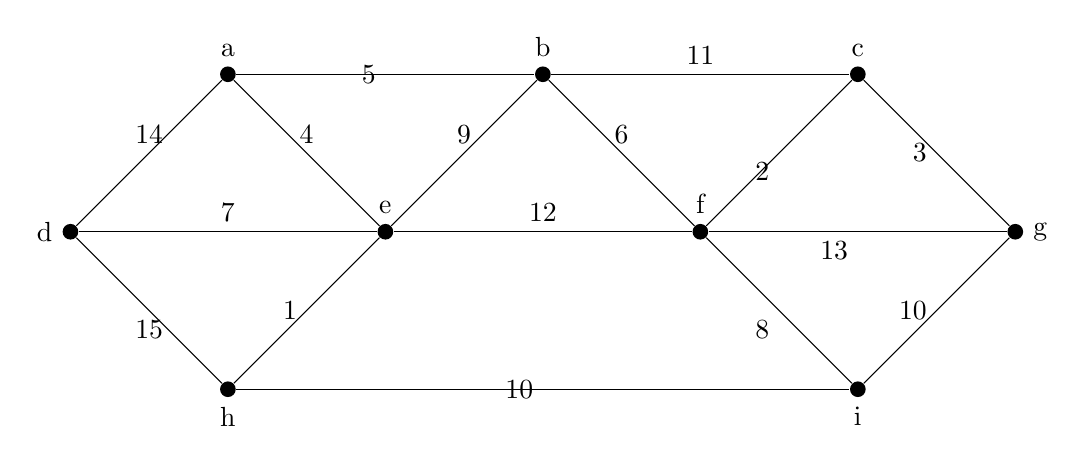
\begin{tikzpicture}
          \node[circle, fill=black, inner sep=2pt, label=left:d] (d)  at (0,2) {};

          \node[circle, fill=black, inner sep=2pt, label=above:a] (a)  at (2,4) {};
          \node[circle, fill=black, inner sep=2pt, label=below:h] (h)  at (2,0) {};
          
          \node[circle, fill=black, inner sep=2pt, label=above:e] (e)  at (4,2) {};

          \node[circle, fill=black, inner sep=2pt, label=above:b] (b) at (6,4) {};
          
          \node[circle, fill=black, inner sep=2pt, label=above:f] (f) at (8,2) {};
          
          \node[circle, fill=black, inner sep=2pt, label=above:c] (c) at (10,4) {};
          \node[circle, fill=black, inner sep=2pt, label=below:i] (i) at (10,0) {};
          
          \node[circle, fill=black, inner sep=2pt, label=right:g] (g) at (12,2) {};
          
          \draw (d) -- (a) node[midway, above] {14};
          \draw (d) -- (e) node[midway, above] {7};
          \draw (d) -- (h) node[midway, below] {15};

          \draw (a) -- (b) node[midway, left] {5};
          \draw (a) -- (e) node[midway, above] {4};
          \draw (h) -- (e) node[midway, left] {1};
          \draw (h) -- (i) node[midway, left] {10};
                
          \draw (e) -- (b) node[midway, above] {9};
          \draw (e) -- (f) node[midway, above] {12};

          \draw (b) -- (c) node[midway, above] {11};
          \draw (b) -- (f) node[midway, above] {6};

          \draw (f) -- (c) node[midway, below left] {2};
          \draw (f) -- (g) node[midway, below left] {13};
          \draw (f) -- (i) node[midway, below left] {8};
          
          \draw (c) -- (g) node[midway, left] {3};
          \draw (i) -- (g) node[midway, left] {10};
        \end{tikzpicture}
        \end{center}
        
        \begin{center}
        \begin{tikzpicture}
          \node[circle, fill=black, inner sep=2pt, label=left:d] (d)  at (0,2) {};

          \node[circle, fill=black, inner sep=2pt, label=above:a] (a)  at (2,4) {};
          \node[circle, fill=black, inner sep=2pt, label=below:h] (h)  at (2,0) {};
          
          \node[circle, fill=black, inner sep=2pt, label=above:e] (e)  at (4,2) {};

          \node[circle, fill=black, inner sep=2pt, label=above:b] (b) at (6,4) {};
          
          \node[circle, fill=black, inner sep=2pt, label=above:f] (f) at (8,2) {};
          
          \node[circle, fill=black, inner sep=2pt, label=above:c] (c) at (10,4) {};
          \node[circle, fill=black, inner sep=2pt, label=below:i] (i) at (10,0) {};
          
          \node[circle, fill=black, inner sep=2pt, label=right:g] (g) at (12,2) {};
          
          \draw (d) -- (e) node[midway, above] {7} node[midway, right] {\textcolor{blue}{7}};

          \draw (a) -- (b) node[midway, left] {5} node[midway, right] {\textcolor{blue}{5}};
          \draw (a) -- (e) node[midway, above] {4} node[midway, right] {\textcolor{blue}{4}};
          \draw (h) -- (e) node[midway, left] {1} node[midway, right] {\textcolor{blue}{1}};
                
          \draw (b) -- (f) node[midway, above] {6} node[midway, right] {\textcolor{blue}{6}};

          \draw (f) -- (c) node[midway, below left] {2} node[midway, right] {\textcolor{blue}{2}};
          \draw (f) -- (i) node[midway, below left] {8} node[midway, right] {\textcolor{blue}{8}};
          
          \draw (c) -- (g) node[midway, left] {3} node[midway, right] {\textcolor{blue}{3}};
        \end{tikzpicture}
        \end{center}

        Gewicht: 36.
\end{enumerate}

\begin{enumerate}[start=58]
  \item Vind een opspannende boom met minimaal gewicht in volgende graaf.
        Geef ook zijn gewicht en de volgorde in dewelke je de bogen vindt.

        \begin{center}
        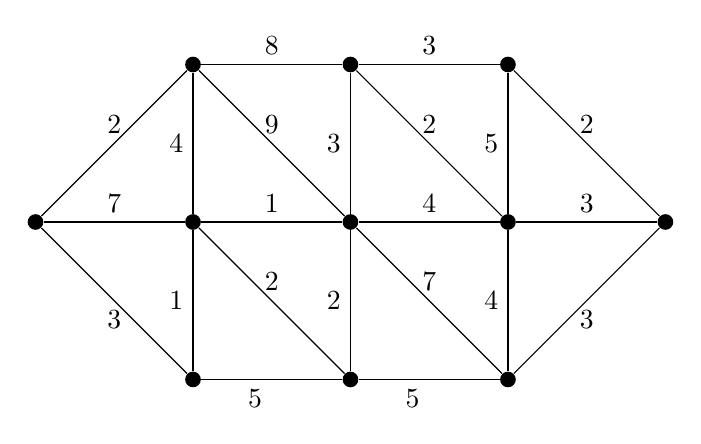
\begin{tikzpicture}
          \node[circle, fill=black, inner sep=2pt] (n1)  at (0,2) {};

          \node[circle, fill=black, inner sep=2pt] (n2)  at (2,0) {};
          \node[circle, fill=black, inner sep=2pt] (n3)  at (2,2) {};
          \node[circle, fill=black, inner sep=2pt] (n4)  at (2,4) {};
          
          \node[circle, fill=black, inner sep=2pt] (n5)  at (4,0) {};
          \node[circle, fill=black, inner sep=2pt] (n6)  at (4,2) {};
          \node[circle, fill=black, inner sep=2pt] (n7)  at (4,4) {};

          \node[circle, fill=black, inner sep=2pt] (n8)  at (6,0) {};
          \node[circle, fill=black, inner sep=2pt] (n9)  at (6,2) {};
          \node[circle, fill=black, inner sep=2pt] (n10) at (6,4) {};
          
          \node[circle, fill=black, inner sep=2pt] (n11) at (8,2) {};
          
          \draw (n1) -- (n4) node[midway, above] {2};
          \draw (n1) -- (n3) node[midway, above] {7};
          \draw (n1) -- (n2) node[midway, below] {3};

          \draw (n3) -- (n4) node[midway, left] {4};
          \draw (n2) -- (n3) node[midway, left] {1};
                
          \draw (n4) -- (n7) node[midway, above] {8};
          \draw (n4) -- (n6) node[midway, above] {9};
          \draw (n3) -- (n6) node[midway, above] {1};
          \draw (n3) -- (n5) node[midway, above] {2};
          \draw (n2) -- (n5) node[midway, below left] {5};
          
          \draw (n6) -- (n7) node[midway, left] {3};
          \draw (n5) -- (n6) node[midway, left] {2};

          \draw (n7) -- (n10) node[midway, above] {3};
          \draw (n7) -- (n9)  node[midway, above] {2};
          \draw (n6) -- (n9)  node[midway, above] {4};
          \draw (n6) -- (n8)  node[midway, above] {7};
          \draw (n5) -- (n8)  node[midway, below left] {5};

          \draw (n9) -- (n10) node[midway, left] {5};
          \draw (n8) -- (n9)  node[midway, left] {4};

          \draw (n10) -- (n11) node[midway, above] {2};
          \draw (n9)  -- (n11) node[midway, above] {3};
          \draw (n8)  -- (n11) node[midway, below] {3};
        \end{tikzpicture}
        \end{center}

        Gierigheidsalgoritme gebruiken: bogen toevoegen in volgorde van gewicht. Bij gelijk gewicht, willekeurig kiezen.
        \begin{center}
        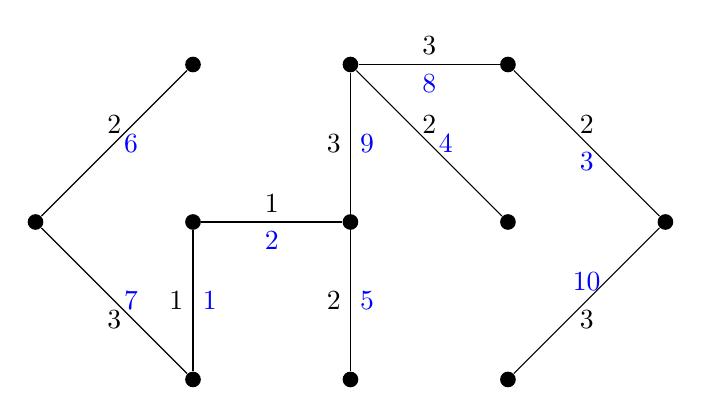
\begin{tikzpicture}
          \node[circle, fill=black, inner sep=2pt] (n1)  at (0,2) {};

          \node[circle, fill=black, inner sep=2pt] (n2)  at (2,0) {};
          \node[circle, fill=black, inner sep=2pt] (n3)  at (2,2) {};
          \node[circle, fill=black, inner sep=2pt] (n4)  at (2,4) {};
          
          \node[circle, fill=black, inner sep=2pt] (n5)  at (4,0) {};
          \node[circle, fill=black, inner sep=2pt] (n6)  at (4,2) {};
          \node[circle, fill=black, inner sep=2pt] (n7)  at (4,4) {};

          \node[circle, fill=black, inner sep=2pt] (n8)  at (6,0) {};
          \node[circle, fill=black, inner sep=2pt] (n9)  at (6,2) {};
          \node[circle, fill=black, inner sep=2pt] (n10) at (6,4) {};
          
          \node[circle, fill=black, inner sep=2pt] (n11) at (8,2) {};
          
          \draw (n1) -- (n4) node[midway, above] {2} node[midway, right] {\textcolor{blue}{6}};
          % \draw (n1) -- (n3) node[midway, above] {7};
          \draw (n1) -- (n2) node[midway, below] {3} node[midway, right] {\textcolor{blue}{7}};

          % \draw (n3) -- (n4) node[midway, left] {4};
          \draw (n2) -- (n3) node[midway, left] {1} node[midway, right] {\textcolor{blue}{1}};
                
          % \draw (n4) -- (n7) node[midway, above] {8};
          % \draw (n4) -- (n6) node[midway, above] {9};
          \draw (n3) -- (n6) node[midway, above] {1} node[midway, below] {\textcolor{blue}{2}};
          % \draw[red, dashed] (n3) -- (n5) node[midway, above] {2};
          % \draw (n2) -- (n5) node[midway, below left] {5};
          
          \draw (n6) -- (n7) node[midway, left] {3} node[midway, right] {\textcolor{blue}{9}};
          \draw (n5) -- (n6) node[midway, left] {2} node[midway, right] {\textcolor{blue}{5}};

          \draw (n7) -- (n10) node[midway, above] {3} node[midway, below] {\textcolor{blue}{8}};
          \draw (n7) -- (n9)  node[midway, above] {2} node[midway, right] {\textcolor{blue}{4}};
          % \draw (n6) -- (n9)  node[midway, above] {4};
          % \draw (n6) -- (n8)  node[midway, above] {7};
          % \draw (n5) -- (n8)  node[midway, below left] {5};

          % \draw (n9) -- (n10) node[midway, left] {5};
          % \draw (n8) -- (n9)  node[midway, left] {4};

          \draw (n10) -- (n11) node[midway, above] {2} node[midway, below] {\textcolor{blue}{3}};
          % \draw (n9)  -- (n11) node[midway, above] {3};
          \draw (n8)  -- (n11) node[midway, below] {3} node[midway, above] {\textcolor{blue}{10}};
        \end{tikzpicture}
        \end{center}

        Na het toevoegen van de 10\textsuperscript{de} boog hebben we een opspannende boom en mogen 
        we het algoritme stoppen. Het minimale gewicht is 22.
\end{enumerate}


\begin{tcolorbox}[title=Methode 2 om planaire graffen te herkennen]
  Stelling van Euler:
  \[ v - e + f = 2\]

  \begin{center}
    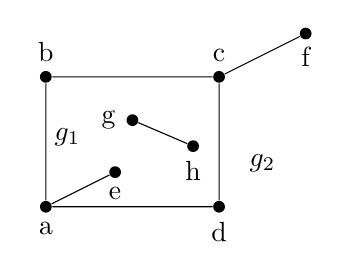
\begin{tikzpicture}[scale=1.1, every node/.style={circle, fill=black, inner sep=1.5pt}]
      \node[label=below:a] (a) at (0,0) {};
      \node[label=above:b] (b) at (0,1.5) {};
      \node[label=above:c] (c) at (2,1.5) {};
      \node[label=below:d] (d) at (2,0) {};
      
      \node[label=below:e] (e) at (0.8,0.4) {};
      \node[label=below:f] (f) at (3  ,2) {};
      \node[label=left :g] (g) at (1  ,1) {};
      \node[label=below:h] (h) at (1.7,0.7) {};

      \node[draw=none, fill=none] (g1) at (0.25, 0.8) {\(g_1\)};
      \node[draw=none, fill=none] (g2) at (2.5, 0.5) {\(g_2\)};

      \draw (a) -- (b) -- (c) --(d) -- (a);
      \draw (a) -- (e);
      \draw (c) -- (f);
      \draw (g) -- (h);

    \end{tikzpicture}
  \end{center}

  Deze planaire graf heeft 2 gebieden: binnen en buiten de rechthoek.

  Op eender welke manier een planaire graf getekend wordt, als het zonder kruisende bogen is, zal het aantal afgetekende
  gebieden (\(f\)) altijd gelijk zijn.

  De rand van een gebied zijn alle bogen waar je op kan botsen. In \(g_1\) kan je botsen op \((a, b), (b, c),(c, d), (d,a)\)
  maar ook op \((a, e)\) en \((g, h)\).

  \(r_{g_1} = 6 \qquad r_{g_2} = 5\)

  \begin{center}
    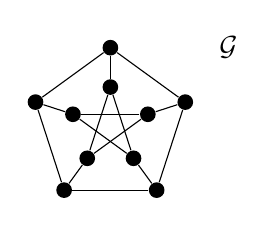
\begin{tikzpicture}
      \begin{scope}
        \node (n) at (1.5, 1) {\(\mathcal{G}\)};
        % Outer pentagon vertices
        \foreach \i in {0,...,4} {
          \node[circle, fill=black, inner sep=2pt] (outer\i) at ({90+\i*72}:1) {};
        }
        
        % Inner pentagon vertices (star pattern)
        \foreach \i in {0,...,4} {
          \node[circle, fill=black, inner sep=2pt] (inner\i) at ({90+\i*72}:0.5) {};
        }
        
        % Outer pentagon edges
        \foreach \i in {0,...,4} {
          \pgfmathsetmacro{\next}{int(mod(\i+1,5))}
          \draw (outer\i) -- (outer\next);
        }
        
        % Inner star edges (each vertex connects to vertex +2 mod 5)
        \foreach \i in {0,...,4} {
          \pgfmathsetmacro{\next}{int(mod(\i+2,5))}
          \draw (inner\i) -- (inner\next);
        }
        
        % Spokes connecting outer to inner
        \foreach \i in {0,...,4} {
          \draw (outer\i) -- (inner\i);
        }
      \end{scope}
    \end{tikzpicture}
  \end{center}

  Stel uit het ongerijmde dat \(\mathcal{G}\) wel planair is.

  \begin{align*}
      v - e + f &= 2 \\
    10 - 15 + f &= 2 \\
              f &= 7
  \end{align*}

  We hebben cycli nodig om het ene gebied af te sluiten van het andere. In een Petersengraaf graf is 
  de kortste cyclus \(c = 5\).

  \begin{gather*}
    35 = 7 \times 5 = \underbrace{\sum_{g \text{ gebied}} 5}_{\text{minstens 5 bogen nodig}} 
    \leq \sum_{g \text{ gebied}} r_g
    \leq \underbrace{2 \times 15}_{\text{een boog kan tot max 2 gebieden horen}} = 30 \\
    35 \not\leq 30
  \end{gather*}
  We komen tot een contradictie, dus \(\mathcal{G}\) is niet planair.

  \textbf{Let op:} het kan zijn dat er geen contradictie uit komt, ook al is de 
                   graf niet planair!
\end{tcolorbox}

\begin{enumerate}[start=62]
  % Oefening 62
  \item Beschouw de gegeven graaf \(\mathcal{G}\).
        \begin{enumerate}
          \item Is dit een Eulergraf? Verklaar.
          \item Toon aan dat G bipartiet is door hem over
                te tekenen op je antwoordblad en de toppen
                z´o te nummeren dat toppen enkel kunnen
                adjacent zijn als hun nummers niet allebei
                even of oneven zijn.
          \item Vind een maximumkoppeling in G. Is dit
                een volledige koppeling?
          \item Wat is de lengte van de kortste cycli in G?
          \item Is deze graaf planair? Geef een bewijs.
        \end{enumerate}

        \hrulefill

        
        \begin{enumerate}[start=5]
          \item Het is een bipartiete graf, dus de kortste cyclus is sowieso even.
                De kortste cyclus is van lengte 6.

                Uit het ongerijmde: de graf is planair, dus:

                \begin{align*}
                    v - e + f &= 2 \\
                  14 - 21 + f &= 2 \\
                            f &= 9 
                \end{align*}

                Het is een drie-reguliere graf, dus \(e = \frac{3 \times 14}{2} = 21\)

                
                \begin{gather*}
                  54 = 9 \times 6 = \underbrace{\sum_{g \text{ gebied}} 6}_{\text{minstens 6 bogen nodig}} 
                  \leq \sum_{g \text{ gebied}} r_g
                  \leq \underbrace{2 \times 21}_{\text{een boog kan tot max 2 gebieden horen}} = 42 \\
                  54 \not\leq 42
                \end{gather*}
        \end{enumerate}
\end{enumerate}

\end{document}